\documentclass[12pt,a4paper]{book}
\usepackage[utf8]{inputenc}
\usepackage[spanish]{babel}

% Paquetes

%\usepackage[nohints]{minitoc}
\usepackage{amsmath}
\usepackage{amsfonts}
\usepackage{amssymb}
\usepackage{amsthm}  % Permite crear teoremas nuevos / Estilos de teoremas 
\usepackage{tikz}
\usepackage{fancybox} % para usar la caja de los ejemplos
\usepackage{subcaption}
\usepackage{wrapfig}
\usepackage{graphicx} 
\usepackage[colorlinks=true,allcolors=blue]{hyperref} % Crea las hiperreferencias (clicas y te mueves) [colorlinks=true,allcolors=blue]
%\graphicspath{ {Figuras/} }
\graphicspath{ {Imagenes/} }


%\theoremstyle{definition}
%\newtheorem{definition}{Definicion}[section]

%\input{structure} % Insert the commands.tex file which contains the majority of the structure behind the templates

\usepackage{fancybox} % para usar la caja de los ejemplos


% Autor y titulo

\title{Apuntes Nanomagnetismo}
\author{Daniel Vázquez Lago}

% Forma del  texto

\setlength{\parindent}{15px}
\usepackage[left=2.25cm,right=2cm,top=4cm,bottom=2cm]{geometry}

% Otros


\numberwithin{equation}{section}
\numberwithin{figure}{section}

% Comandos propios
\newcommand{\tquad}{\quad \quad \quad}

\newcommand{\parentesis}[1]{\left( #1  \right)}
\newcommand{\parciales}[2]{\frac{\partial #1}{\partial #2}}
\newcommand{\pparciales}[2]{\parentesis{\parciales{#1}{#2}}}
\newcommand{\ccorchetes}[1]{\left[ #1  \right]}
\newcommand{\D}{\mathrm{d}}
\newcommand{\derivadas}[2]{\frac{\D #1}{\D #2}}

\newcommand{\Tr}{\mathrm{Tr} \ }
\newcommand{\eV}{\mathrm{eV}}
\newcommand{\cte}{\mathrm{cte}}
\newcommand{\eff}{\mathrm{eff}}
\newcommand{\mf}{\mathrm{mf}}


\newcommand{\Hcal}{\mathcal{H}}
\newcommand{\Jsf}{\mathsf{J}}


% Comandos vectoriales

\newcommand{\xn}{\mathbf{x}}
\newcommand{\yn}{\mathbf{y}}
\newcommand{\zn}{\mathbf{z}}
\newcommand{\vn}{\mathbf{v}}
\newcommand{\un}{\mathbf{u}}
\newcommand{\rn}{\mathbf{r}}
\newcommand{\qn}{\mathbf{q}}
\newcommand{\pn}{\mathbf{p}}
\newcommand{\kn}{\mathbf{k}}
\newcommand{\sn}{\mathbf{s}}
\newcommand{\an}{\mathbf{a}}
\newcommand{\bn}{\mathbf{b}}
\newcommand{\nn}{\mathbf{n}}
\newcommand{\mn}{\mathbf{n}}
\newcommand{\lnn}{\mathbf{l}}

\newcommand{\An}{\mathbf{A}}
\newcommand{\Bn}{\mathbf{B}}
\newcommand{\En}{\mathbf{E}}
\newcommand{\Jn}{\mathbf{J}}
\newcommand{\Hn}{\mathbf{H}}
\newcommand{\Ln}{\mathbf{L}}
\newcommand{\Mn}{\mathbf{M}}
\newcommand{\Pn}{\mathbf{P}}
\newcommand{\Sn}{\mathbf{S}}

\newcommand{\mun}{\boldsymbol{\mu}}
\newcommand{\rhon}{\boldsymbol{\rho}}

% Comandos vectoriales unitarios

\newcommand{\hrho}{\hat{\rhon}}
\newcommand{\hnu}{\hat{\un}}
\newcommand{\hns}{\hat{\sn}}
\newcommand{\hnr}{\hat{\rn}}
\newcommand{\hnx}{\hat{\xn}}
\newcommand{\hny}{\hat{\yn}}
\newcommand{\hnz}{\hat{\zn}}

% Comandos teoremas

\newtheorem{theorem}{Teorema}[section]
\newtheorem{definition}{Definicion}[section]


% Comandos teoremas


\begin{document}

\maketitle


\newpage


\tableofcontents % Print the table of contents itself

\newpage

%\chapter{Introducción}

%Este libro habla sobre la manifestación del magnetismo en la materia condenada (líquidos y sólidos). Los solidos contienen momentos magnéticos que pueden interactuar constructivamente entre ellos. En función de la interacción entre los momentos magnéticos tendremos unos comportamientos u otros. Esto es lo que genera la cantidad de propiedades magnéticas en sistemas reales. En este capítulo introductorio recopilaremos los conocimientos básicos de los momentos magnéticos en la electrodináimca clásica y la mecánica cuántica. 

%\section{Momentos magnéticos}
%\subsection{Momentos magnéticos y momentos angulares}
%\subsection{Precesión}
%\subsection{Magnetón de Bohr}
%\subsection{Magnetización y campo}

%\section{Mecánica clásica y momentos magnéticos}
%\subsection{Momentos canónicas}
%\subsection{El Bohr-Van Leeuwen teorema}

%\section{Mecánica Cuántica del Espín}
%\subsection{Momento magnético orbital y de espín}
%\subsection{Matrices de Pauli}
%\subsection{Operadores escalera}
%\subsection{Acoplamiento de dos espines}

%\newpage

%\chapterimage{T-02.jpeg} % Chapter heading image

\newpage
    Hola a todos. Este son unos apuntes incompletos hechos en el curos 2023/2024 por Daniel Vazquez Lago, basandose (prácticamente parafraseando y traduciendo) el Blundell, por lo que faltarán detalles de Javier Castro, otros libros que también usa el... Como algunos habreis visto dejo en la carpeta un archivo zip con el código de \LaTeX y las imagenes usadas (la mayoría de cosecha mía, las otras son de algunos libros, aunque teneis permiso explícito para usarlas libremente) para que podais ampliar y mejorar estos temas que faltan, así como corregir erratas (que debe haber docenas) y, en general, mejorar estos apuntes. De no funcionar no dudeis en contactar conmigo a traavés de mis correos daniel.vazquez.lago@rai.usc.es o danielvazquezlago@gmail.com. Un saludo, y mucha suerte con todo.
\newpage

\chapter{Momentos mangéticos aislados}

En este capítulo vamos a tratar la propiedad de magnéticos aislados. En este nivel, las interacciones entre diferentes momentos magnéticos de diferentes átomos y sus alrededores serán ignorados. Nosotros queremos conocer la física de átomos aislados, y su inter
acción en presencia de un campo magnético externo. Por supuesto eso no implica que vaya a ser sencillo, simplemente que la dificultad tendrá una naturaleza diferente a la de temas posteriores. 

\section{Átomo en presencia de un campo magnético}

Para entender como interacciona un átomo en presencia de un campo mangético primero debemos hallar la forma de su hamiltoniano. La energía debida al espín de un electrón en presencia de un campo magnéitco paralelo al eje $z$ viene dada por:

\begin{equation}
E = g \mu_B B m_s
\end{equation}
donde $g \approx 2$, $m_s = \pm \frac{1}{2}$. Entonces $E \approx \pm \mu_B B$. Además del momento angular espín, los electrones también poseen un momento angular orbital. Si la posición de nuestro electrón $i$ es $\rn_i$, con momento $\pn_i$ y momento angular total $\hbar \Ln$:

\begin{equation}
\hbar \Ln = \sum_i \rn_i \times \pn_i
\end{equation}
donde la suma se hace respecto todos los electrones del átomo. Además debemos considerar el hamiltoniano $H_0$ dado por:

\begin{equation}
\Hcal_0 = \sum_{i=1}^Z \parentesis{\frac{p_i^2}{2m} + V_i}
\end{equation}
donde $V_i$ es la energía potencial del electrón $i$, y $p_i/2m$ su energía cinética (no relativista). Podemos asumir sin ningún tipo de problema que $H_0$ tiene autovectores y autovalores conocidos. Además debemos añadir la energía dada por el potencial magnético. Para un campo magnético constante en una dirección determinada $\Bn = B \hnz$, siempre podremos encontrar gauge que verifique que el potencial magnético del electrón $i$ venga dado por 

\begin{equation}
\An_i = \frac{\Bn \times \rn_i}{2}
\end{equation}
En ese caso tenemos que:

\begin{equation}
\Hcal = \Hcal_0 + \mu_B (\Ln  + g \Sn) \cdot \Bn + \frac{e^2}{8 m_e} \sum_i (\Bn \times \rn_i)^2
\end{equation}

La perturbación \textit{dominante} del hamiltoniano es $\Hcal_0 \sim 10$eV. El segundo término y tercer término son perturbaciones significativamente menores, pero suficientes como para que aparezcan los fenómenos del paramangétismo y diamagnetismo. De hecho al término $\mu_B (\Ln  + g \Sn) \cdot \Bn $ se le llama el \textbf{término paramagnético} y al término $\frac{e^2}{8 m_e} \sum_i (\Bn \times \rn_i)^2$ el \textbf{término diamagnético}. El término paramangético será mucho mas grande que el término diamagnético (un orden de diferencia de $10^{-4}$).

\section{Susceptibilidad magnética}

La susceptibilidad magnética para un medio lineal viene dada por $\Mn = \chi \Hn$ donde $\Mn$ es el momento magnético por unidad de volumen (también llamada magnetización). Según esta definición de magnetización $\chi$ representa el momento magnético inducido por un campo magnético imanador $\Hn$ \textit{por unidad de volumen}, aunque sea adimensional.   \\

Muchas veces se usa la suscetibliidad magnética por mol ($\chi_m = \chi V_m$) o  por unidad de masa ($\chi_g = \chi / \rho$). Si la suscetibilidad magnética es negativa llamamos al material un material \textit{diamangético} y si el material es un material con una susceptibilidad positiva un material \textit{paramangético}.

\section{Diamagnetismo}

Todos los materiales presentan cierto grado de \textbf{diagmagnetismo}, esto es, una débil susceptibilidad magnética negativa. Para una substancia diamangética tenemos que el campo magnético inducido se \textit{opone} al campo magnético aplicado que lo causa. \\

Este efecto a veces trata de explicarse usando la mecánica clásica: la acción de un campo magnético sobre un electrón ``orbitando'' causa una fuerza electromotriz inducida que dada la ley de Lenz se opone al campo magnético que la produce. Aunque pueda entenderse así, este modelo no es suficiente como para predecir la naturaleza del diamagnetismo. Esto se debe a que dicho fenómeno es puramente cuántico, y como tal debe ser tratado desde la mecánica cuántica. \\

Consideremos el caso de un átomo que tenga todos las capas rellenas (esto hace que $\Ln = 0$ y $\Sn = 0$) de tal manera que el término paramagnético se anule. Ahora el término de primer orden $\Delta E$ para el estado fundamental (en ingles \textit{ground state}) será el término diamagnético. Si nuestro campo magnético es paralelo al eje $z$ tal que $(\Bn \times \rn_i)^2 = B^2 (x_i^2+y_i^2)$

\begin{equation}
\Delta E_0 = \frac{e^2 B^2}{8 m_e} \sum_{i=1}^Z \langle 0 | (x_i^2+y_i^2) | 0 \rangle 
\end{equation}
donde $|0\rangle$ es el estado fundamental de la función de ondas. Dado que  que podemos asumir una simetría esférica (para $J=0$ asumir la simetría esférica es considerada una buena aproximación) tenemos que $\langle x_i^2 \rangle = \langle y_i^2 \rangle = \frac{1}{3} \langle r_i^2 \rangle$, por lo que:

\begin{equation}
\Delta E_0 = \frac{e^2 B^2}{12 m_e} \sum_{i=1}^Z \langle 0 | (r_i^2) | 0 \rangle 
\end{equation}
Considerando un sólido de $N$ iones (con una masa de $m$ y $Z$ electrones) en un volumen $V$ (con todas sus capas llenas), y usando que la definición termodinámica-estadística de la magnetización (a $T=0$) es la derivada de la energía libre de Helmholtz ($F$) respecto el campo mangético, podemos obtener que la magenitzación es:

\begin{equation}
M = - \parciales{F}{B} = - \frac{N}{V} \parciales{\Delta E_0}{B} = - \frac{N e^2 B}{6 m_e} \sum_{i=1}^Z \langle r_i^2 \rangle
\end{equation}
y por tanto si $\chi = M / H \approx \mu_0 M / B$ (tal que $\chi << 1$), tenemos que el resultado es

\begin{equation}
\chi = - \frac{N}{V} \frac{ e^2 \mu_0}{6 m_e} \sum_{i=1}^Z \langle r_i^2 \rangle \label{Ec:02-03-004}
\end{equation}
Esta expresión asume una aproximación a primer orden. A medida que la temperatura de la substancia aumente, también aumentará la energía del estado fundamental, haciendo que este cada vez sea mas relevante en detrimento del momento magnético.   \\

El término diamagnético aparece en cualquier tipo de material, por lo que es muy relevante su estudio. Es la presencia de otros fenómenos, como el paramagnetismo la que pueden opacarlo, pero eso no implica que se apague.

%\begin{exercise}
%Calcula la susceptibilidad diamangética de un gas de átomos de hidrógenos con $n=10^{20} \ \mathrm{m}^{-3}$ en el estado fundamental.  
%\end{exercise}
%\begin{solution}
%Para calcular dicho término asumimos que $\langle r_i^2 \rangle = a_B^2/3$, donde $a_B=10$pm es el radio de Bohr. Para el campo $B=1$T, como solo tenemos un electrón en cada átomo $(Z=1)$, tendremos que nuestra energía viene dada por

%$$ \Delta E_0 = \frac{e^2 B^2}{12 m_e} a_B^2 \sim 10^{-9} \mathrm{eV} $$
%La susceptibilidad electromagnética, en virtud de la ecuación \ref{Ec:02-03-004} tendremos que vale:
%$$ \chi_{dia} = - \frac{N}{V} \frac{e^2 \mu_0}{6 m_e} a_0^2 = -1.65 \cdot 10^{-16} $$
%\end{solution}


\section{Paramagnetismo}

El paramagnetismo corresponde a la susceptibilidad magnétoca positiva, por lo que un campo magnético induce una mangetización paralela al campo magnético que la causa. En la sección previa hemos considerado un átomo o ión que no contiene electrones no emparejados. Solo en presencia de un campo magnético externo aparecerá un momento magnético no nulo.  \\

En este apartado estudiaremos átomos con un momento magnético no nulo debido precisamente a estos electrones no desapareados. Siempre que no apliquemos un campo magnético podemos considerar que estos momentos magnéticos son completamente independientes, y que apuntan cada uno a un lugar aleatorio, siendo su valor medio  cero. Es la aplicación del campo magnético lo que causa su alineación (lógicamente en función de la intensidad del campo) manifestado así los efectos paramagnéticos.  Será fundamental el \textbf{momento angular total} $\Jn$ del átomo, que es la suma del momento angular orbital y el momento angular espín.:

\begin{equation}
    \Jn = \Ln + \Sn
\end{equation}

Aunque un incremento del campo magnético tienda alinear los momentos magnéticos, un incremento de la temperatura tenderá a desalinearlos. Es de esperar entonces que la magnetización venga dada de alguna forma del ratio $B/T$. Como veremos a continuación, el paramagnetismo es un fenómeno mucho mas fuerte que el fenómeno diamagnético.


\subsection{Aproximación semi-clásica}

El tratamiento semi-clásico del paramagnetismo ignora completamente el hecho de que los momentos magnéticos tienen restringido las direcciones a donde pueden apuntar (en la mecánica clásica pueden apuntar en cualquier dirección) debida a la cuantización. \\

Vamos a considerar un material a una temperatura $T$ no nula, por lo que habrá que tener en cuenta la mecánica estadística. Nos interesa calcular que proporcion del momento magnético medio apunta en la dirección del campo mangético $\Bn$, esto es, nos interesa calcular $\langle \mu_z \rangle$. Para calcular el valor medio simplemente tenemos que integrar:

$$  \langle \mu_z \rangle = \iint \mu \cos (\theta) P (\theta,T)  \D \Omega $$
donde $\mu$ es el \textbf{momento magnético} de dicho átomo, tal que $\mun = g_l \Ln + g_s \Sn $ donde $g_l$ y $g_s$ son los factores giromangéticos. Dado que estamos trabajando con temperatura, si suponemos que nuestro material está en contacto con un termostato a temperatura constante y uniforme (distribución canónica) , tal y como puede ser un océano, o el aire de una habitación; tendremos que usar los factores de Boltzmann tal que:

\begin{equation}
P (\theta,B) = \frac{\exp \parentesis{E(\theta)/k_B T}}{\int \exp\parentesis{E(\theta)/k_B T} \D \Omega}
\end{equation} 
siendo el determinante el factor de normalización. Dado que la energía $E(\theta) = \mun \cdot \Bn = \mu B \cos \theta$, tenemos finalmente que:

\begin{equation}
\langle \mu_z \rangle = \frac{\int_0^\pi \mu \cos (\theta) \exp \parentesis{\mu B \cos (\theta) / k_B T} \sin \theta \D \theta}{\int_0^\pi \exp \parentesis{\mu B \cos (\theta) / k_B T} \sin \theta \D \theta}
\end{equation}
para solucionar la integral sugerimos el cambio de variable $x=\cos \theta$, y $y=\mu B / k_B T$ (este último para simplificar los resultados). La solución final es la \textbf{función de Langevin} $L(y)$, que usando las variables anteriores viene dada por:

\begin{equation}
\langle \mu_z \rangle \equiv \mu \ccorchetes{\coth y - \frac{1}{y}} \equiv L(y)
\end{equation}
si $y$ es pequeño, podemos realizar la aproximación de segundo orden tal que

$$\coth (y) = \frac{1}{y} + \frac{y}{3} + \mathcal{O} (y^3)$$
Denotamos por $n$ al número de momentos magnéticos por unidad de volumen. La \textbf{saturación magnética}, $M_s$, es la máxima magnetización que podemos obtener, ya que en este caso todos los momentos magnéticos están alineados ($M_s = n \mu$). De esta manera tenemso que la magnetización viene dada por:

\begin{equation}
\frac{M}{M_s} = \frac{\langle \mu_z \rangle}{\mu} \approx \frac{y}{3} = \frac{\mu B}{3 k_B T}
\end{equation}
de lo que obtenemos la susceptibilidad mangética $\chi = M/H \approx \mu_0 M / B$ (válida para campos pequeños, con $chi << 1$) tal que:

\begin{equation}
\chi = \frac{n \mu_0 \mu^2}{3 k_B T}
\end{equation}
lo que demuestra que la \textit{susceptibilidad magnética es inversamente proporcional a la temperatura}, la llamada \textbf{ley de Curie}. 

\subsection{Paramagnetismo para $J=1/2$}

El cálculo anterior servirá ahora para introducir para un sistema cuántico. Si cambiamos los momentos clásicos por momentos de espín cuánticos $J=1/2$, solo con dos posibles valores en el eje $z$, tal que $m_J = \pm \frac{1}{2}$. Esto es: puede ser paralelo o antiparalelo a $B$. Así con obtenemos que:

\begin{equation}
\langle g \mu_B m_J \rangle = \frac{- \mu_B e^{-mu_B B / k_B T}+\mu_B e^{mu_B B / k_B T}}{e^{-mu_B B / k_B T}+e^{mu_B B / k_B T}}
\end{equation}
de esta manera tenemos que (usando $g \approx 2, \ J=1/2$):

\begin{equation}
\frac{M}{M_S} = \frac{\langle m_J \rangle}{J} = \tanh (y)
\end{equation}
Que es diferente a la función de Langevin (aunque parecida). Esto nos lleba a que para campos pequeños tal que $\tanh (y) = y + \mathcal{O}(y^2)$, obtener la susceptibilidad

\begin{equation}
\chi = \frac{n \mu_0 \mu_B^2}{k_B T}
\end{equation}

\subsection{Función de Brilluoin}

El caso general, donde $J$ puede ser un entero o un semi-entero va a ser calculado en este apartado. Los dos casos mas comunes (que son $J = \infty$ y $J=1/2$) estarán contenidos en este caso general, y lógicamente serán recuperables. Como vamos a ver un campo magnético creciente tenderá a alinear los momentos magnéticos y un incremiento de la temperatura tenderá a desalinearlos. \\

Lo primero que debemos hacer es estudiar la función de partición usada anteriormente, ya que contiene toda la información termodinámico-estadística del sistema. La razón por la que es vital su estudio es porque en ella está incluida la probabilidad de que encontremos un estado con determinada energía (remitimos a la mecánica estadística para entender mejor el concepto). La \textbf{función de partición} vendrá dada entonces por:

\begin{equation}
Z = \sum_{m_J=-J}^{J} \exp \parentesis{m_J g_J \mu_B B / k_B T} = \sum_{m_J=-J}^{J} \exp \parentesis{m_J x}
\label{Ec:02-04-009}
\end{equation}
donde hemos hecho el cambio de variables $x=g_J \mu_B B / k_B T$, tendremos que el momento magnético medio en la dirección $z$ vendrá dado por:

\begin{equation}
\langle m_J \rangle = \frac{\sum_{m_J} m_J e^{m_J x}}{\sum_{m_J} e^{m_J x}} = \frac{1}{Z}  \parciales{Z}{x}
\end{equation}
Dado que este es el momento magnético medio de una partícula, la magnetización de un cuerpo (donde $n=N/V$, la densidad de partículas) viene dada por:

\begin{equation}
M = n g_J \mu_B \langle m_J \rangle = \frac{n g_J \mu_B}{Z} \parciales{Z}{B} \parciales{B}{x} = n k_B T \parciales{\ln (Z)}{B}
\end{equation} 
Ahora bien, se puede ver como la función de partición (ecuación \ref{Ec:02-04-009}) no es más que una \textit{serie geométrica y}  de $2J$ miembros, con un término inicial $a=e^{-Jx}$, y por razón tiene a $r = e^x$. De este modo tenemos que si una serie geométrica con términos que viene dada por:

$$ \sum_{j=1}^M a r^{j-1} = \frac{a (1-r^M)}{1-r} $$
donde $M=2J+1$. Obtenemos entonces que la \textbf{función de partición} viene dada, tras unas pequeñas manipulaciones puramente algebráicas, por

\begin{equation}
Z = \frac{\sinh \ccorchetes{(2J+1)\frac{x}{2}}}{\sinh \ccorchetes{\frac{x}{2}}}
\end{equation}
Ahora resulta evidente el anterior enunciado: conocida la función podemos conocer todas las variables termodinámicas puestas en juego, incluso la magnetización y el momento magnético medio. De este modo, tras derivar, podemos obtener que:

\begin{equation}
M = M_S B_J (y) \tquad y = x J = g_J \mu_B J B / k_B T
\end{equation}
siendo $M_S$ la \textbf{magnetización de saturación}, que no es más que la magnetización máxima que nuestro sistema puede alcanzar (se obtiene suponiendo que todos los momentos magnéticos están alineados), y siendo $B_J$ la \textbf{función de Brilluoin}. Ambos están definidos por:

\begin{equation}
    M_S = n g_J \mu_B J
\end{equation}

\begin{equation}
    B_J (y) = \frac{2J+1}{2J} \coth \parentesis{\frac{2J +1}{2J} y} - \frac{1}{2J} \coth \parentesis{\frac{y}{2J}}
\end{equation}
En la figura \ref{Fig:02-04-01} podemos observar una gráfica con $B_J(y)$ para diferentes valores de $J$. Como podemos observar, si llevamos al límite clásico ($J\rightarrow \infty$, haciendo continuo el momento magnético) la ecuación,  obtendremos la \textit{función de Langevin}:

\begin{equation}
    B_{\infty} (y) = L(y)
\end{equation}
Si llevamos la funció de Brillouin al límite cuántico ($J=1/2$), obtendremos la ecuación tanh, tal que

\begin{equation}
    B_{1/2} (y) = \tanh(y)
\end{equation}
obteniendo el mismo resultado que en los apartados previos, demostrando que el desarrollo termodinámico es consistente. Si usamos la aproximación $\chi \ll 1$, cierta para cuando el campo no es muy intenso ($B \approx 1$T) y/o temperaturas extremadamente grandes ($T=293$K), obtenemos que $y\approx 2\cdot 10^{-3}$. Para un valor de $y$ pequeño como el anterior ($y \ll 1$, y consecuentemente $\chi \ll 1$) podemos usar la expansión de Maclaurin para el $\coth (y)$, obteniendo la aproximación

\begin{equation}
B_J (y) = \frac{(J+1)y}{3J} + \mathcal{O} (y^3)
\end{equation}
de tal modo que la susceptibiliad mangética $\chi$ pueda aproximarse por

\begin{equation}
\chi =\frac{M}{H} \approx \frac{\mu_0 M}{B} = \frac{n \mu_0 \mu_{eff}^3}{3 k_B T}
\end{equation}
El valor de $\chi$ nos permite deducir el valor del \textit{momento magnético efectivo} de un átomo donde $\mu_{\eff}$ viene determinado por

\begin{equation}
\mu_{\eff} = g_J \mu_B \sqrt{J (J+1)} \tquad g_J = \frac{3}{2} + \frac{S(S+1)-L(L+1)}{2J(J+1)}
\end{equation}
siendo $g_J$ el llamado \textbf{valor g de Landé}. La ley de Curie de la dependencia de la susceptibilidad magnética nos lleva a qeu $\chi \varpropto 1/T$. Esto es muy útil sobretodo para futuros capítulos donde consideraremos el rol de todas estas interacciones mangéticas.  \\

Es muy interesante ver uqe $\mu_\eff$ coincide con $\mu$ (siendo $\mu = M_S/n$) únicamente cuando $J\rightarrow \infty$. Esto contiene una información del sistema muy relevante: únicamente cuando el momento mangético es clásico le es lícito al campo mangético efectivo (esto es, el campo magnético medido medio) tener el valor máximo posible del momento magnético $\mu$. Esto se puede explicar mediante el principio de inceritdumbre de Heisenberg.

\begin{figure}[h!]
    \centering
    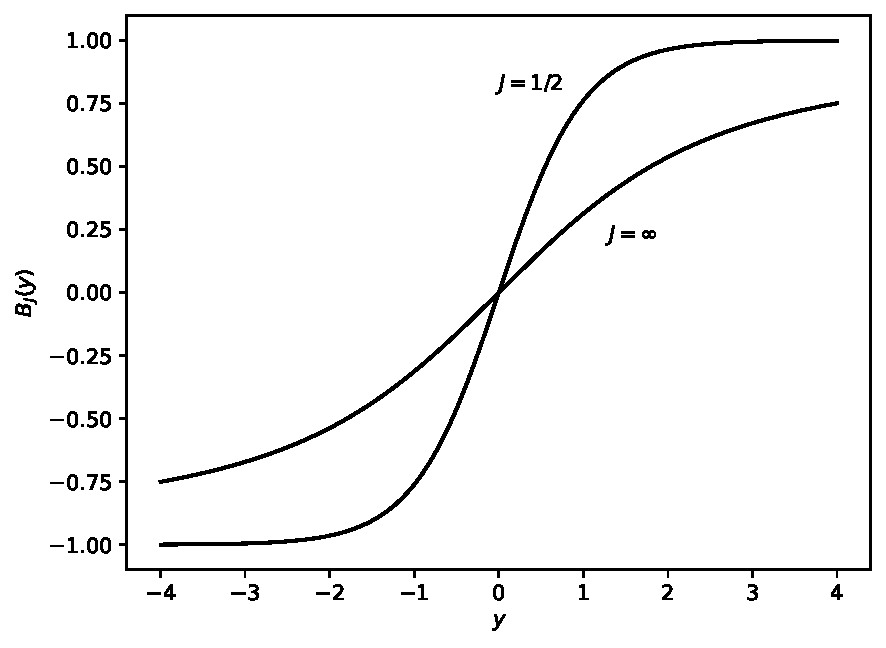
\includegraphics{Imagenes/02-Brillouin.pdf}
    \caption[scale=1]{función de Brilluoin.}
    \label{Fig:02-04-01}
\end{figure}

\subsection{Paramagnetismo de Van Vleck}

Si $J=0$ esto implica que el estado fundamental $|0\rangle$, y que por tanto no haya paramagnetismo, ya que

\begin{equation}
    \langle 0 | \mun | 0 \rangle = g_J \mu_B \langle 0 | \Jn |0 \rangle = 0
\end{equation}
Esto implica que la energía del sistema no cambia si el campo magnético es aplicado, y por tanto no hay susceptibilidad mangética debido a fenómenos paramagnéticos. Sin embargo esta conclusión es válida únicamente para una \textit{perturbación de primer orden}. Una perturbación a segundo orden precide que existe un cambio de la energía del estado fundamental $\Delta E_0$ porque esta tiene lugar en estados excitados tales que $J\neq 0$. El cambio de energía respecto el estado fundamental $\Delta E_0$ debido a esto viene dado por:

\begin{equation}
    \Delta E_0 = \sum_n \parentesis{ \frac{|\langle 0 |(L_z + g S_z)|n\rangle|^2}{E_0 - E_n} } - \frac{e^2}{8 m_e} \sum_i (\Bn \times \rn_i)^2
\end{equation}
siendo el priemr término debido a todos los estados excitados del sistema, y el segundo término debido al diamagnetismo. Entonces la susceptibilidad magnética viene dada por

\begin{equation}
    \chi = \frac{N}{V} \parentesis{ 2\mu_B \sum_n \parentesis{ \frac{|\langle 0 |(L_z + g S_z)|n\rangle|^2}{E_n - E_0} } - \frac{e^2 \mu_0}{6 m_e} \sum_i \langle r_i^2 \rangle }
\end{equation}
Al primer término se le llama \textbf{paramagnetismo de Van Vleck}, y es positivo al verificarse que $E_n>E_0$. El paramagnetismo de Van Vleck es muy débil, al igual que el diamagnetismo. 

\section{Estado fundamental del ion y las reglas de Hund}

Un átomo típico contiene varios electrones. Muchos de estos estarán en orbitales llenos que no aportan momento angular neto. Sin embargo si que puede haber electrones presentes en orbitales no llenos, pudiendo generar un momento angular orbital o de espín no nulo. \\

Las diferentes configuraciones de momentos magnéticos orbitales y de espín son las que hacen que, los electrones al tratar de colocarse en los orbitales, tengan energías diferntes. La diferencia de energía entre colocarse en un orbital u otro viene determinada por la elección de momento angular de espín, que afecta a una parte de la función de ondas; y el momento angular orbital, que afecta a como los electrones se mueven alrededor del núcleo. Por eso vamos a tratar, en esta sección, de buscar cuál es la configuración que minimiza esta energía

\subsection{Reglas de Hund}

La combinación de los números cuánticos angulares que minimizan la energía pueden ser estimadas usando las \textbf{reglas de Hund}. Estas tres reglas empíricas estan ordenadas en función del orden de relevancia. 

\begin{enumerate}
    \item Primero trataremos de \textit{maximizar el espín} $S$. Debido al principio de exclusión de Pauli, que nos dice que dos electrones con el mismo espín deben ser tener funciones de onda espaciales ortogonales. Asi se reduce la repulsión entre electrones. 

    \item Para la función de ondas dada por la anterior regla, el siguiente paso es \textit{maximizar el momento angular orbital} $L$. Dos electrones orbitanddo tienen menos probabilidades de encontrarse si giran en la misma dirección. 

    \item Finalmente se tratará de \textit{minimizar la relación espín-orbita}. El valor de $J$ vendrá dado por la relación $J=|L-S|$ si el orbital está medio vacío, y por $J=|L+S|$ si el orbital está medio lleno. Como podemos ver, esta regla solo se puede aplicar en ciertas circustancias. Por ejemplo en los metales de transición, las energías de espín-órbita no son mucho mas grandes qeu otros términos como el campo cristalino, por lo que esta regla debería desobedecerse. Por otro lado, para las tierras raras esta regla funciona sumamente bien. \\
\end{enumerate}

Denotamos por $^{2S+1}L_J$ al término que nos dice los números cuánticos $S,L,J$ para cierto átomo. Es importante decir que $L$ no se da como un número, si no como una letra, dada por la tabla \ref{Tab:02-05-01}.

\begin{table}[h!] 
    \centering
    \begin{tabular}{c|cccccccc}
       L  & 0 & 1 & 2 & 3 & 4 & 5 & 6 & $ \cdots $  \\ \hline
          & S & P & D & F & G & H & I & $ \cdots $ 
    \end{tabular}
    \caption{relación símbolo-número cuántico}
    \label{Tab:02-05-01}
\end{table}




%\subsection{L-S y acoplamiento j-j}

%\section{Desmagnetización adiabática}
%\section{Espín nuclear}
%\section{Estructura hiperfina}

\newpage

\chapter{Entorno}

Como hemos visto en el capítulo anterior, las propiedades magnéticas de muchos cristales que contengan tierras raras pueden ser deducidas suponiendo que los iones de tierras raras no interaccionan entre sí. Sin embargo para ciertos iones magnéticos, en algunos cristales, uno no puede ignorar ciertas interacciones, y para algunos materiales estas son suficientemente grandes para considerarlas. En este capítulo consideraresmso las interacciones entre el átomo y sus vecinos mas inmediatas. \\

\section{Campos cristalinos}

Para entender el efecto del entorno local debido a los niveles de energía de los átomos, es necesario en primer lugar ver un poco como son los tamaños y formas de los orbitales atómicos. ünicamente los orbitales $s$ son esféricos, el resto tienen una dependencia angular acusada. Esto es crucial, ya que es son los entornos locales no esféricos lo que hacen que los orbitales se comporten de una manera tan diferente.

\subsection{Origen de los campos cristalinos}

Un campo cristalino es un campo eléctrico debido al efecto de átomos vecinos en el cristal. En la \textbf{teoría de campos cristalinos} los orbitales vecinos son modelados como cargas putuales negativas. Una mejora de esta aproximación es la \textbf{teoría de campos ligados}, que es esencialmente una extensión de la teoría orbital molecular que se centra en el rol de los orbitales $d$ respecto el ion central, y su superposición con orbitales vecinos llamados \textit{ligandos}. El tamaño y naturaleza del cristal depende esencialmente de la simetría del entorno local. Un caso común es considerar un entorno local octaédrico. Esto es porque en muchos metales de transición los iones se colocan en el centro con un ion como puede ser el oxígeno en cada uno de las esquinas. En este caso el campo cristalino se manifiesta como la repulsión electroestática negativa debido a los electrones cargados negativamente. \\

\subsection{Bloqueo orbital}

El momento magnético esperado para los estados fundamentales $3d$ no siguen el momento predicho por $g_J[J(J+1)]^{1/2}$,. La razón por la que suceden estas discrepancias es que las interacciones de campos  cristalinos son mucho mas fuertes que las interacciones espín-órbita. De este modo la tercera regla de Hund, basa directamente en estas interacciones espín-órbita, pasa a ser incorrecta. Los datos experimentales coinciden con los teóricos si se supone que $L=0$, esto es, $J=S$ con $g_J = 2$. Así

\begin{equation}
    \mu_{\eff} = 2 \mu_B \sqrt{S(S+1)}
\end{equation}
A este efecto donde el momento agular parece desaparecer se le llama \textbf{extición orbital} o \textbf{bloqueo orbital} (del inglés \textit{orbital queching}). Para los iones $4f$, donde los orbitales están mucho mas cerca del núcleo, entre los obitales $5s$ y $5p$, por lo que el campo cristalino tendrá una influencia mucho menor. Por esa misma razón estos átomos si verifican la tercera ley de Hund. El caso de los metales de transición $4d$ y $5d$ es bastante ambiguo, ya que si presentan una interacción de campo cristalino, pero mucho menos intensa que la de los orbitales $3d$. \\

La razón por la cuál existe este bloqueo de momento angular es que los campos cristalinos en los iones $d$ son mucho mas fuertes que la interacción espín-órbit, de tal modo que pasará a ser una interacción perturvativa (de segundo orden). Esto se debe a que los autoestados del hamiltoniano en las estrucutas cristalinas son puramente reales, mientras que el operador $\Ln \equiv i\hnr \times \nabla$ es puramente imaginario. Dado que $\Ln$ es un operador hermítico, y el resultado de aplicar el operador sobre una función de ondas real debe ser un valor real, la única posibilidad es que sea cero (sobre el estado fundamental). De existir perturbaciones que alteren el estado fundamental, la interacción de espín-órbita dejaría de ser nula y debería ser considerada, pero precisamente como una interacción de segundo orden.  


%\subsection{El efecto Jahn-Teller}

%\section{Técnicas de resonancia magnéticas}
%\subsection{Resonancia nuclear magnética}
%\subsection{Resonancia del espín del electrón}
%\subsection{Espectroscopía de Mössbauer}
%\subsection{Rotación del espín del muon}


\newpage
\chapter{Interacciones}

En este capítulo vamos a considerar diferentes tipo de interacciones magnéticas que pueden ser importantes a la hora de las interacciones magnéticas de largo alcance, ya que permitirán que los diferentes mometos magnéticos de un sólido se comuniquen entre sí.

\section{Interacción dipolar magnética}

La primera interacción que esperamos que aparezca con un rol importante es la \textbf{interacción magnética dipolar}. Dos dipolos magnéticos $\mun_1$ y $\mun_2$ separados por una distancia $\rn$ tienen una energía igual a

\begin{equation}
    E = \frac{\mu_0}{4 \pi r^2} \ccorchetes{\mun_1 \cdot \mun_2 - \frac{3}{r^2} (\mun_1 \cdot \rn) (\mun_2 \cdot \rn)}
\end{equation}

Como podemos ver esta interacción depende del grado de separación entre los momentos y el grado de alineamiento entre ambos. Se pueden estimar fácilmente suponiendo que $\mu \approx \mu_B$ con $r \approx 1 \text{\r{A}}$. En ese caso la energía $\mu^2 / 4 \pi r^3 \sim 10^{-23} \text{J}$. Esta energía es la energía equivalente a $k_BT$ con $T=1 \mathrm{K}$. En general no encontraremos metales a esta temperatura, estarán a una mucho mayor, por lo que esta interacción será demasiado débil para el orden que estamos buscando. \\

\section{Interacción de permutación}

Las \textbf{interacciones de intercambio} o \textbf{energías de permutación} (la traducción de \textit{exchange interactions} permite ambas acepciones) son el corazón del fenómeno de las \textit{interacciones a largo alcance}. Escoger el término permutación en vez de intercambio revela una física mucho más profunda que decir intercambio. En el siguiente apartado veremos el porqué. Como todo el magnetismo, este fenómeno es un fenómeno cuántico, más concretamente son el fruto de interacciones electrostáticas. La razón por la que se llaman energías de permutación o energías de permutaciones precisamente radican

\subsection{Origen de la permutación}
Sean dos electrones, uno de ellos ocupando la posición $\rn_1$ y el otro ocupando la posición $\rn_2$. La energía triplete $E_T$ y las energía singlete $E_S$ son las energías asociadas a los estados triplete  $\Psi_T$ y singlete $\Psi_S$ respectivamente, tal que

\begin{equation}
    E_S = \int \Psi_S^* \Hcal \Psi_S \D \rn_1 \D \rn_2
\end{equation}
\begin{equation}
    E_T = \int \Psi_T^* \Hcal \Psi_T \D \rn_1 \D \rn_2
\end{equation}
Ahora podemos ver el porque de la elección de la palabra permutación en nuestra traducción. Es la necesidad de que la permutación entre electrones (al ser indistinguibles) genere un signo negativo debido a su naturaleza de fermión la que nos obliga a que la \textit{función de ondas global sea antisimétrica}, y por tanto la que genera las diferentes energías. Definimos la \textbf{constante de permutación} $\mathsf{J}$ (también llamada integral de permutación) como:

\begin{equation}
    \Jsf = \frac{E_S - E_T}{2} = \int \psi_a^* (\rn_1) \psi_b^* (\rn_2) \Hcal \psi_a (\rn_2) \psi_b (\rn_1) \D \rn_1 \D \rn_2
\end{equation}
de esta manera el \textit{hamiltoniano efectivo} entre dos electrones puede ser escrito como
\begin{equation}
    \Hcal = - 2 \Jsf \Sn_1 \cdot \Sn_2 \label{Ec:04-02-05}
\end{equation}
Si $\Jsf>0$ tenemos que se favorecerá el estado triplete ($S=1$) ya que $E_S>E_T$. Si $\Jsf<0$ se favorecerá el estado singlete ($S=0$) ya que $E_S<E_T$. En cualquier caso esta ecuación es relativamente sencilla para dos electrones, pero difícil de generalizar para un sistema extenso. Dada la dificilutad de su generalización, ya en los primeros días de la mecánica cuántica se supuso que las interacciones de un átomo se pueden reducir a las interacciones con sus vecinos. En ese caso tendremos el \textbf{modelo de Heisenberg} para el hamiltoniano:

\begin{equation}
    \Hcal =- \sum_{ij} \Jsf_{ij} \Sn_i \cdot \Sn_j \label{Ec:04-02-005}
\end{equation}
donde $\Jsf_{ij}$ es la constante de permutación entre el espín número $i$ y el espín número $j$. El factor 2 es omitido porque el sumatorio ya incluye cada par de espines. \\

El cálculo de la integral puede ser complicada en general. Por esa misma razón vamos a introducir algunos conceptos. En primer lugar, si dos electrones son del mismo átomo, la integral de permutación es normalmente positiva. Esto estabiliza el estado triplete y se asegura que los electrones sean antisimetricos espacialmente, lo que minimiza la repulsión de Coulomb entre ambos electrones (mantieniéndolos lo más separado posible). Esto es consistente con la primera regla de Hund. \\

Cuando los dos electrones son de átomos vecinos, la situación es muy diferente. Cualquier estado será la combinación de un electrón centrado en un átomo y otro electrón centrado en el otro átomo. Esto hace que la energía de los electrones se parezca a la energía de una partícula encerrada en una ``caja'' unidimensional de tamaño $L$. Dicha energía va con la inversa del cuadrado del tamaño de la caja ($L^{-2}$). Esto nos permite relacionar una mayor energía cinética con una caja más pequeña. Así los elecgtrones tratarán de formar enlaces de tal manera que puedan moverse por ambos átomos, esto es, una ``caja más grande'', lo que les permitirá tener una energía cinética mas pequeña. A estos estados se les llama \textbf{orbitales moleculares}. Los estados que se pueden formar son los \textbf{estados enlazantes} espacialmente simétricos (en ingles \textit{bounding states}) y los \textbf{estados antienlazantes} que son espacialmente antisimétricos (en ingles \textit{antibounding states}). Estos últimos son energéticamente más costosos. Esto favorece el estado singlete, con espín $S=0$.

\subsection{Permutación directa}

Si los electrones de átomos vecinos interaccionan mediante la interacción de permutación decimos que hay \textbf{permutación directa} o \textbf{intercambio directo.} Se dice directo porque la permtuación sucede sin ningún tipo de intermediario. Aunque este sea la ruta mas obvia para que la interacción de permutación tenga lugar, la realidad física no suele ser tan sencilla. \\

En muchas ocasiones nos encotramos que la permutación directa no es el mecanismomas importantes a la hora de entender las propiedades magnéticas de un metal. ¿La razón? Que no hay suficente superposición entre los orbitales magnéticos. Por ejemplo, en los electrones $4f$ de las tierras raras están fuertemente localizadas cerca del núcleo, por lo que la probabildiad de que la densidad de probabilidad se extienda hasta el espacio interatómico. Esto significa que la permutación direta es poco usual en las teirras raras. Incluso en los metales como el hierro, cobalto y níquel, los orbitales $3d$ no se extienen lo suficiente como para que la permutación directa permita explicar las propiedades magnéticas de los mismos. Que estos materiales sean metales implica que la conductividad eléctrica no debe ser ignorada, por lo que una correcta descripción de los mismos necesitará tener en cuenta las bandas de electrones. Debido a esto para entender muchos de los materiales magnéticos es necesario tener en consideración algún tipo de \textbf{interacción de permutación indirecta.}

\subsection{Permutación indirecta en sólidos iones: superpermutación}

La \textbf{superpermutación} sucede cuando, entre dos iones magnéticos existe un ión no magnético, que permite hacer que la interacción de intercambio, en general de muy corto alcance, aumente su radio de efectividad. Por eso el nombre de súper, ya que es una interacción de largo alcance. Este fenómeno se puede encontrar en los óxidos o fluoruros de manganeso (MnO, MnF$_2$).  \\

Las \textbf{reglas de Goodenouh-Kanamori-Anderson} \footnote{Visitar la página http://www.scholarpedia.org/article/Goodenough-Kanamori\_rule} son un conjunto de reglas que nos permiten deducir las propiedades magnéticas de un material donde halla una interacción de superintercambio, en base al ángulo entre los orbitales atómicos, el tipo de orbitales atómicos en interacción, si están medio llenos o medio vacíos... Así podremos deducir a priori si un material es ferromagnético o antiferromagnético. Las reglas son \footnote{Pedro Cacheda}:

\begin{enumerate}
    \item El intercambio a 180º entre orbitales llenos es ferromagnético y relativamente fuerte.
    \item El interacambio a 90º entre orbitales casi llenos es ferromagnético y relativamente débil. 
    \item Cuando el solapamiento sucede entre un orbital vacío y otro ocupado, la interacción es ferromagnética y relativamente débil. 
\end{enumerate}

%\subsection{Permutación indirecta en metales}


%\subsection{Doble permutación}
%\subsection{Interacción de permutación anisótropa}
%\subsection{Aproximación al continuo}


\newpage

\chapter{Orden y estructuras magnéticas}

En los capítulos anteriores hemos presentado diferentes tipos de interacciones magnéticas entre diferentes momentos magnéticos en un sólido. En este capítulo vamos a consierar los diferentes tipos de interacciones magnéticas que pueden oucrrir en el \textit{estado fundametal} de un sólido. Los estados fundamentales incluyen las interacciones \textbf{ferromagnéticas} (todos los momentos magnéticos están alineados) y \textbf{antiferromagnéticas} (los momentos magnéticos son antiparalelos respecto sus adyacentes). Además veremos las estructuras helicoidales, espirales y las giratorias (en la literatura inglesa las \textit{spin glasses}). En este capítulo nos preocuparemos por enseñar como todas las interacciones previamente mencionadas nos permiten diferentar estos estados fundamentales, y como el fenómeno del orden es una consecuencia de la rotura de simetría. 

\section{Ferromagnetismo}

Un \textbf{material ferromagnético} (FM) tiene una magnetización espontánea incluso en ausencia de un campo magnético externo. Esto se debe a que todos los momoentos magnéticos apuntan en una única dirección \footnote{En la realidad lo que ocurre es que el material mangético se divide en regiones llamadas dominios, en las cuales los momentos magnéticos si apuntan en la misma dirección, aunque entre dominions puede que la dirección si llegue a diferir.}. Este efecto se debe a las interacciones de permutación mencionadas en el apartado anterior. Para un FM en presencia de un campo externo $\Bn$ tendrá un hamiltoniano tal que:

\begin{equation}
    \Hcal = - \sum_{ij} \Jsf_{ij} \Sn_i \cdot \Sn_j + g \mu_B \sum_j \Sn_j \cdot \Bn \label{Ec:05-01-001}
\end{equation}
donde las constantes de permutación entre los vecinos serán positivas, ya que en caso contrario los espines serían antiparalelos. Como podemos ver la ecuación \ref{Ec:05-01-001}, el primer término es la energía de intercambio de Heinserberg (ecuación \ref{Ec:04-02-005}) y la segundo término la energía de Zeeman. 

\subsection{El modelo de Weiss de un material ferromagnético}

Para tratar de resolver la ecuación \ref{Ec:05-01-001} vamos a definir el \textbf{campo mangético molecular} ($\Bn_\mf$ de \textit{molecular field}) efectivo, dado por

\begin{equation}
    \Bn_{\mf} = -\frac{2}{g \mu_B} \sum_j \Jsf_{ij} \Sn_j \label{Ec:05-01-002}
\end{equation}
Dado que la energía de Zeeman viene dada por $g \mu_B \Sn_i \cdot \Bn_i$, tenemso que el término de Heinsenberg se puede remplazar por $g \mu_B \sum_i \Sn_i \cdot \Bn_\eff$. En ese caso el hamiltoniano se podrá escribir como

\begin{equation}
    \Hcal = g \mu_B \sum_i \Sn_i \cdot (\Bn + \Bn_\mf) \label{Ec:05-01-003}
\end{equation}
que luce como un hamiltoniano de un material paramagnético en un campo externo $\Bn + \Bn_\mf$. El supuesto que sustenta este enfoque es que todos los iones experimentan el mismo campo magnético molecular. Esto es, ciertamente, cuestionable, particularmente para temperaturas cerca de la transición magnética. Para un campo ferromagnético el campo molecular actuará para alinear los momentos magnéticos vecinos. Esto sucede precisamente por que la energía de permutación es positiva. \\

Dado que el campo molecular mide el grado de orden del sistema de los diferentes momentos magnéticos podemos asumir una relación lineal entre $\Bn_\mf$ y $\Mn$ parametrizada por una constante $\lambda$ 

\begin{equation}
    \Bn_\mf = \lambda \Mn \label{Ec:05-01-004}
\end{equation}
como podemos ver $\lambda$ es una constante que parametriza la fuerza del campo magnético como función de la mangnetización. Para un material ferromagnético $\lambda>0$. Debido a la gran energía de Coulomb implicada en la energía de permutación tenemos que el campo mmolecular suele ser extremadamente grande en los materiales ferromangéticos. \\

Ahora seremos capaces de tratar el problema del ferromagnetismo como un problema paramagnético pero con un campo magnético $\Bn+\Bn_\mf$. Para bajas temperaturas el momento puede está alineado con el campo magnético molecular, incluso sin aplicar un campo magnético externo $\Bn$. Uno debe darse cuenta de que es el alineamiento entre moléculas el que permite la aparcición de este campo molecular magnético, siendo a su vez este el responsable del propio alineamiento. \\

En cualquier caso a baja temperatura el ordenamiento magnético es capaz de mantenerse por si mismo. Es para temperaturas cada vez mayores cuando las fluctuaciones térmicas comienzan progresivamente a destruir la mangetización, hasta que llegue la \textit{temperatura crítica} donde todo tipo de orden magnético quedará destruido. A este modelo se le llama el \textbf{modelo ferromagnético de Weiss}. para encontrar soluciones de este modelo debemos solucionar simultaneamente las ecuacioens 

\begin{equation}
    \frac{M}{M_s} = B_J (y) \tquad y = \frac{g_J \mu_B J (B+\lambda M)}{k_B T} \label{Ec:05-01-005}
\end{equation}
Restrinjámonos de momento al caso $B=0$. Estas ecuaciones pueden ser resueltas gráficamente. Para esto debemos graficar ambas ecuaciones y buscar el punto en el que se cortan. Definimos como \textbf{temperatura crítica} o \textbf{temperatura de Curie} $T_C$ aquella temperatura para la cual la \textit{única solución} del sistema es $M=0$. Como $M\rightarrow0$, tenemos que $y\ll 1$, podemos usar la aproximación de la función de Brillouin $B_J = (J+1)y/3J$. En ese caso podemos ver que a ambos lados de la ecuación $\frac{M}{M_S}=B_J(y)$ aparece $M$. Cancelando ambos términos entre sí podemos obtener  que:

\begin{equation}
    T_C= \frac{g_J \mu_B (J+1) \lambda M_s}{3 k_B} = \frac{n \lambda \mu_\eff^2}{3 k_B}
\end{equation}
En la figura podemos ver que si $T>T_C$ \textit{no existe solución}, y si $T<T_C$ \textit{existen dos soluciones} de igual valor absoluto diferente signo $\pm M(T_0)$. Lógicamente la curva también de $J$. De hecho podemos graficar cuales son las soluciones del sistema de ecuaciones en función de $(J,T/T_C)$ obteniendo una familia de curvas. \\

\begin{figure}[h!]
    \centering
    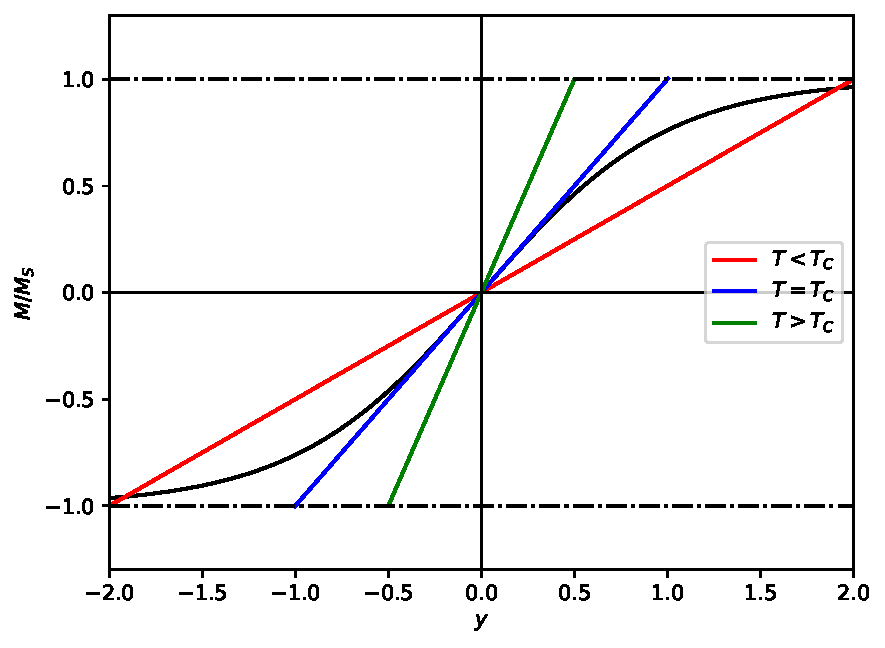
\includegraphics[scale=1]{Imagenes/05-TC.pdf}
    \caption{solución gráfica al sistema de ecuaciones.}
    \label{Fig:05-01-01}
\end{figure}


Volviendo a la temperatura de Curie. Como podemos ver dihca temperatura nos da un valor teórico para el cual el fenómeno del ferromagnetismo desaparece. Esto no es mas que la temperatura para la cual sucede la \textbf{transición de fase de segundo orden} entre el ferromagnetismo y el no-magnetismo. Substituyendo $\lambda M_S$ por $B_\mf$, podremos obtener el valor del campo magnético efectivo (si conocemos el valor de la temperatura crítica y $J$). En ese caso

\begin{equation}
    B_\mf = \frac{k_B T_C}{\mu_B g_J (J+1)}
\end{equation}
un valor típico de $T_C \sim 10^3K$ y $J=1/2$ nos da un valor del campo magnético molecular $B_\mf \approx 1500$T. Como podemos ver es un campo enorme, lo que refleja la fuerza de la energía de permutación. 

\begin{figure}[h!]
    \centering
    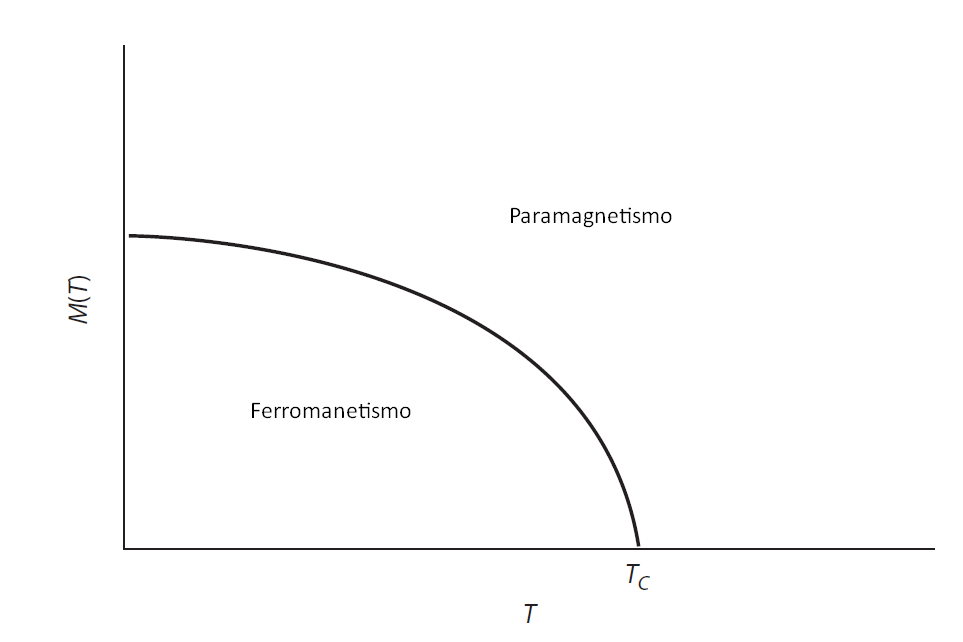
\includegraphics[scale=0.6]{05-Ferro.png}
    \caption{Valor de $M/M_S$ en función de $T$.}
    \label{Fig:05-01-02}
\end{figure}

\subsection{Susceptibilidad magnética}

Si aplicamos un campo magnético externo $B$ (pequeño) para $T\geq T_C$, obtendremos un valor pequeño de la magnetización (y lo que es lo mismo, $y\ll 1$). En ese caso la aproximación de la función de Brillouin será válida, de tal modo que

\begin{equation}
    \frac{M}{M_S} \approx \frac{g_J \mu_B (J+1)}{3k_B} \parentesis{\frac{B+\lambda M}{T}} 
\end{equation}
de tal modo que:

\begin{equation}
    \frac{M}{M_S} \parentesis{1-\frac{T_C}{T}} \approx \frac{T_C B}{\lambda M_S}
\end{equation}
obteniendo así la conocida \textbf{ley de Curie Weiss}:

\begin{equation}
    \chi = \lim_{B \rightarrow 0} \frac{\mu_0 M}{B} \varpropto \frac{1}{T-T_C}
\end{equation}

\begin{figure}[h!]
    \centering
    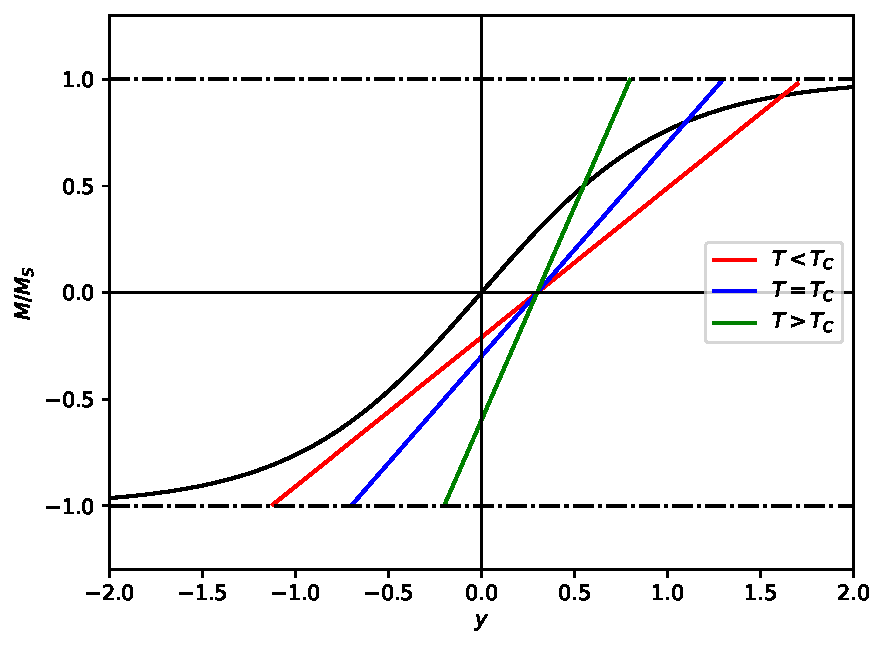
\includegraphics[scale=1]{05-TC-B.pdf}
    \caption{solución gráfica al sistema de ecuaciones con $B\neq 0$.}
    \label{Fig:05-01-03}
\end{figure}




\subsection{El efecto de un campo magnético}

Tal y como puede verse en la figura \ref{Fig:05-01-03}, el efecto de añadir un campo magnético nulo lo que hace es mover el centro de las rectcas. Esto hace que para cualquier temperatura exista una solución, y por tanto la transición de fase se cancele. Para materiales ferromagnéticos en presencia de un campo magnético no nulo, siempre existirá algún tipo de ventaja energética que permita este alineamiento. En este modelo n oes necesario considerar el efecto de un campo magnético apuntando en diferentes direcciones. En la dirección  que apunte el campo magnético también apuntará la magnetización inducida. El modelo no contiene una dirección espacial privilegiada. En un material ferromagnético esto \textit{no es cierto}, por lo que existe algún tipo de anisotropia magnética que deberá ser considerada (siguiente capítulo).  \\

A la temperatura $T=T_C$, la temperatura es suficientemente grande como para suponer que $B_J=(J+1)y/3J -\zeta y^3math + \mathcal{O} (y^5)$ donde $\zeta$ es una constante. Para resolver esto tenemos que:

\begin{equation}
    y = \frac{g_J \mu_B J (B+\lambda M)}{k_B T_C} = \frac{(B+\lambda M)}{\zeta M_s}
\end{equation}
de tal modo que

\begin{equation}
    M = M_S \zeta \frac{(B+\lambda M)}{\lambda} - \zeta \parentesis{\frac{3J(B+\lambda M)}{\lambda (J+1) M_S}}^3
\end{equation}
de lo que se demuestra que:

\begin{equation}
    B \varpropto (B+\lambda M)^3
\end{equation}
de tal modo que si se verifica la relación $\lambda M \gg B$, tenemso que el término de la derecha pasa a ser dominado por $M^3$, tal que $M \varpropto B^{1/3}$.


\subsection{El origen del campo molecular}

Cuando Weiss (1907) propuso el modelo magnético molecular se sintió decepcionado al ver que $\lambda$ debía ser muy grande para los valores grandes de $T_C$ que realmente se encuentran en la naturaleza. No era posible suponiendo un origen dipolar de los mismos (recordemos que $B_\mf = 10^3T$). Fue con Heisenberg y su modelo, que involucraba directamente las enormes energías de Coulomb, lo que pudo explicar como se generaba un campo tan grande. \\

De esta manera el campo molecular parametrizado por $\lambda$ puede ser relacionado con la energía de permutación $\Jsf_{ij}$. Asumimos que la energía de permutación es efectiva únicamente sobre el eje $z$ sobre los vecinos del ion estudiado. Usando las ecuaciones anteriores 

\begin{equation}
    \lambda = \frac{2z\Jsf}{n g^2 \mu_B^2} \label{Ec:05-01-014}
\end{equation}
entonces la temperatura de Curie puede ser calculada como

\begin{equation}
    T_C = \frac{2z \Jsf J(J+1)}{3k_B}
\end{equation}

En toda nuestra disertación hemos asumido que $L=0$ y por tanto que $J=S$. Esto funciona para casi todos los iones $3d$, ya que, como hemos explicado en capítulos anteriores, en estos iones sucede la extición orbital. \\

Sin embargo para los iones $4f$, $\Sn$ deja de ser un buen número cuántico, y $\Jn$ pasa a ser uno bueno. Dado que $\Jn=\Ln+\Sn$, y $g_J \Jn = \Ln + 2 \Sn$, tendremos que un buen número cuántico es $(g_J-1)\Jn$. Consecuentemente $\Sn$ en la expresión \ref{Ec:05-01-001} debe ser substituido por $(g_J-1)\Jn$. Repitiendo de manera exacta el mismo procedimiento podemos llegar a que

\begin{equation}
    \lambda = \frac{2 z \Jsf (g_J-1)^2}{n g_J^2 \mu_B^2} \label{Ec:05-01-016}
\end{equation}
Para el caso de metales de transición donde $g_J=2$, podmeos ver que la ecuación \ref{Ec:05-01-016} se reduce en la ecuación \ref{Ec:05-01-014}. El factor de temperatura crítica es propircional entonces al conodico \textbf{factor de Gennes} $(g_J-1)^2J(J+1)$.  

\section{Antiferromagnetismo}

Si la energía de intercambio es negativa, $\Jsf<0$, el campo molecular esta orientado de tal manera que es favorable a los momentos magnéticos más cercanos ser antiparalelos. A esto se le llama \textbf{antiferromagnetismo}. En muchas ocasiones estos sistemas pueden estudiarse como dos \textbf{subredes}. En una de las subredes el campos magnéticos apuntará hacia arriba, y en la otra hacia abajo. En un primer lugar supondremos que el campo molecular de una subred es proporcional a la magnetiaación de la otra subred. Además asumiremos que no hay campo magnético aplicado. 


\begin{figure}[h!]
    \centering
    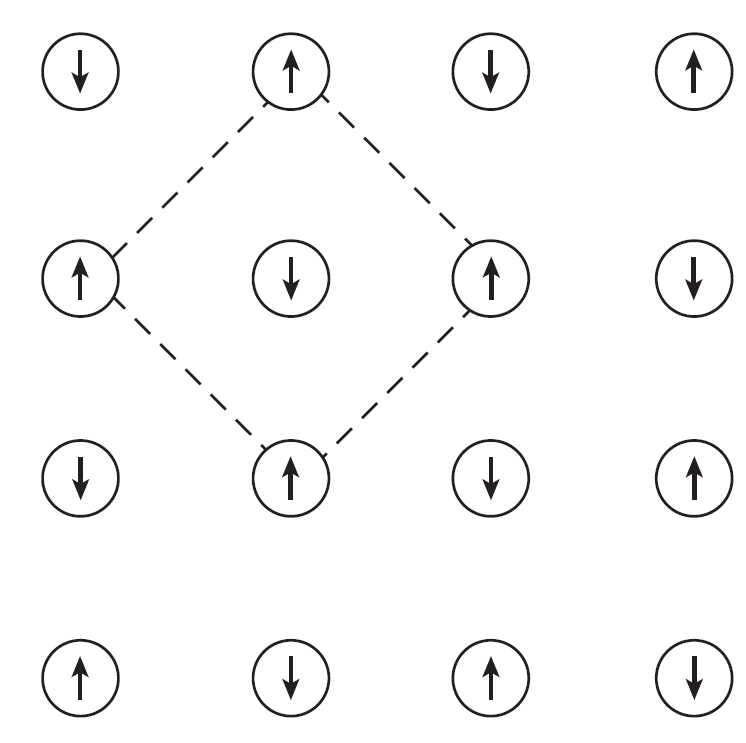
\includegraphics[scale=0.6]{05-Subred.png}
    \caption{}
    \label{Fig:05-02-01}
\end{figure}

\subsection{Modelo de Weiss del antiferromagnetismo}

Si suponemos que la subred $+$ apunta hacia ``arriba'', y la subres $-$ apunta hacia abajo, entonces el campo molecular de cada subred es:

\begin{equation}
    \begin{array}{lll}
        B_+ & = & - |\lambda|M_{-}  \\
        B_{-} & = & - |\lambda|M_+ 
    \end{array}
\end{equation}
donde $\lambda$ es el campo molecular constante que ahora es negativo. En cada subred el campo molecular vendrá dado por:

\begin{equation}
    M_\pm = M_S B_J \parentesis{- \frac{g_J \mu_B J |\lambda | M_\mp}{k_B T}}
\end{equation}
dado que las magnetizaciones de cada subred son iguales salvo en la orientación, tememos que

\begin{equation}
    |\Mn_+|=|\Mn_-| = \Mn
\end{equation}
de tal modo que

\begin{equation}
    M = M_S B_J \parentesis{\frac{g_J \mu_B J |\lambda| M}{k_B T}}
\end{equation}
que, como podemos ver, es prácticamente idéntica a las ecuaciones del ferromagnetismo \ref{Ec:05-01-005}, por lo que la fomra es la misma. La temperatura de transición, a partir la cual el antiferromagnetismo desaparece, es la llamada \textbf{temeraptura de Néel} $T_N$, definida por

\begin{equation}
    T_N = \frac{g_J \mu_B (J+1) |\lambda|M_S}{3k_B} = \frac{n |\lambda|\mu^2_{\eff}}{3k_B} \label{Ec:05-02-005}
\end{equation}
dado que ambas magnetizaciones apuntan en direcciones opuestas, la suma neta de ambas $M_+ + M_-$ será cero. Uno puede definir la llamada \textbf{magnetización escalonada} como la diferencia de ambas $M_+-M_-$. Esta no es nula para temperaturas debajo de $T_N$, por lo que puede ser usada como parámetro de orden para los materiales antiferromagnéticos. 

\subsection{Susceptibildad magnética}

\begin{figure}[t]
    \centering
    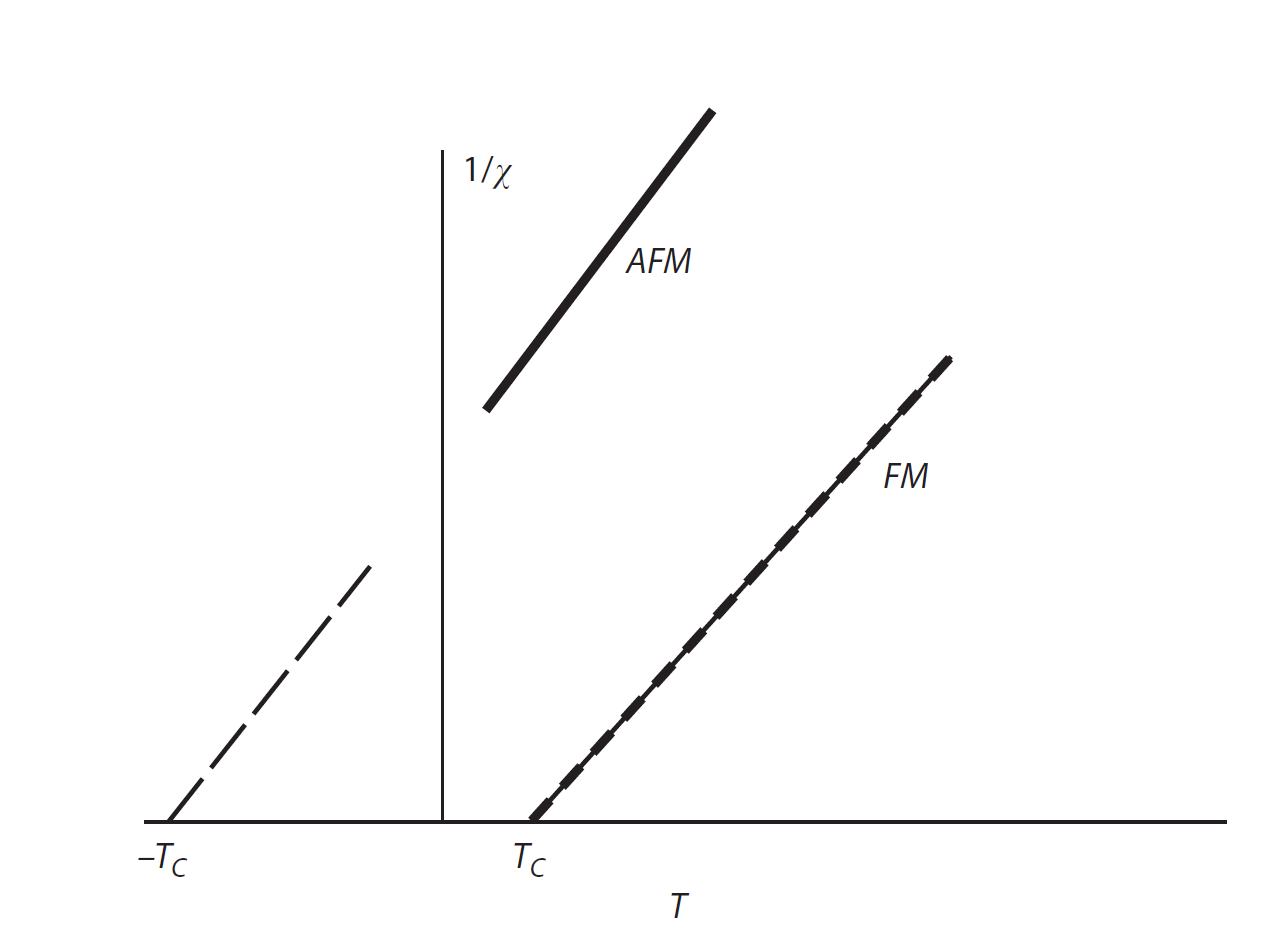
\includegraphics[scale=0.5]{05-LeyWeiss.png}
    \caption{ley de Weiss en función de $\theta$}
    \label{Fig:05-02-02}
\end{figure}

Para temperaturas superiores a $T_N$ el efecto de aplicar un campo magnético externo pequeño sobre nuestro material puede ser calculado del mismo modo que en el caso de un material ferromagnético, expandiendo la función de Brillouin $B_J(y)=(J+1)y/3J + \mathcal{O}(y^3)$. Así podríamso obtener la susceptibilidad magnética:

\begin{equation}
    \chi \varpropto \frac{1}{T+T_N}
\end{equation}
Esto es, la ley de Curie-Weiss pero ahora el término $-T_C$ será remplazado por el término $+T_N$. Este resultado nos permite clasificar los materiales en un estado paramagnético usando precismanete la ley de Curie-Weiss. Si la susceptibilidad magnética va con 

\begin{equation}
    \chi \varpropto \frac{1}{T - \theta}
\end{equation}
tendremos la siguiente clasifiación: 
\begin{itemize}
    \item Si $\theta>0$ el material será \textbf{ferromagnético}. 
    
    \item Si $\theta=0$ el material será \textbf{paramagnético}.
    
    \item Si $\theta<0$ el material será \textbf{antiferromangético}. 
\end{itemize} 

Experimentalmente la temperatura $\theta$ para los materiales antiferromangéticos estan muy lejas de las temperaturas de Neel predichas predichas por la ecuación \ref{Ec:05-02-005}. Esta discrepancia es razonable, ya que hemos supuesto que el campo magnético de una subred depende únicamente de la magnetización de la otra subred. En la figura \ref{Fig:05-02-02} \\


Aplicando un campo mangético al material antiferromagnético a temperaturas inferiores a la $T_N$ produce efectos mas complicados que para el caso feromagnético. La razón es el fenómeno depende de la  \textit{dirección} en la que se aplique el campo. Para ver un poco como funciona este fenómeno, consideremos primero que estamos en el cero absoluto (o cerca de el) tal que así la agitación térmica pueda ser ignorada. En ese caso $|M_+|=|M_-|=M_S$. Si un campo mangético pequeño es aplicado en la dirección de las subredes, el efecto neto es cero ya que los términos que aparecerían en ambas subredes se cancelaría entre sí, tal que $\chi_{||} = 0$. Si en lugar de aplicar el campo magnético en la dirección perpendicular a las subredes, tendremos que la magnetización de cada una de las subredes girará un ángulo $\phi$ tratando de hacerse paralelo con el campo aplicado. Aunque el efecto neto en la dirección paralela a las subredes siga siendo nulo, aparecerá un término en la dirección perpendicular no nulo, tal que $\chi_T \neq 0$. Esto puede verse en \\

Si la temperatura ahora se aumenta (mateniéndonos aún en $T<T_N$) tendremos que las flucutaciones térmicas disminuirán el campo molecular en cada subred. Esto afecta a la susceptibilidad $\chi_{||}$, no a la susceptibilidad magnética perpendicular, que es independiente de la temperatura. \\

\begin{figure}
    \centering
    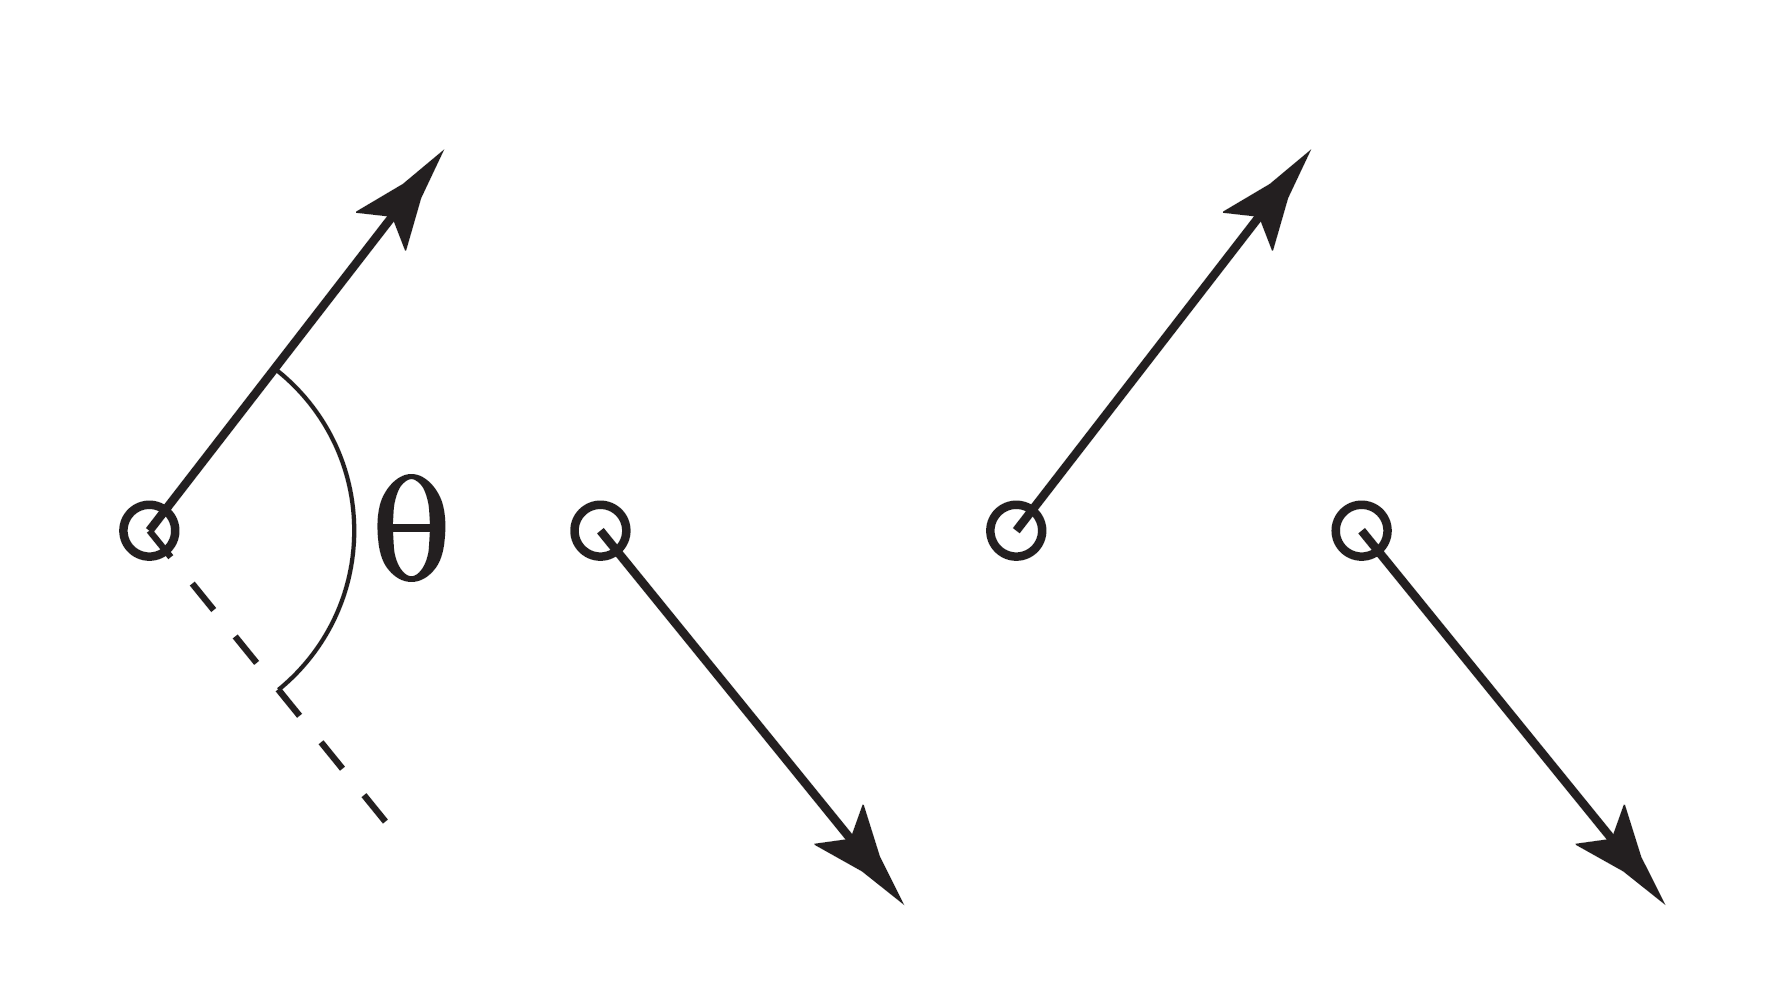
\includegraphics[scale=0.3]{05-Antiferro.png}
    \caption{momentos magnéticos al acplicar un campo magnético perpendicular.}
    \label{Fig:05-02-03}
\end{figure}

%\subsection{Efecto de un campo mangético fuerte}

%\subsection{Tipos de orden antiferromagnético}

\section{Ferrimagnetismo}

El tratamiento del antiferromagnetismo asume que existen dos subredes equivalentes entre sí. La pregunta que nos hacemos ahora es: ¿Qué pasaría si no son equivalentes? Si no fueran iguales u opuestas, entonces existirá una magnetización enta. A este fenómeno se le llama \textbf{ferrimagnetismo}. Debido a qeu el campo molecular en cada subred es diferente, la magnetización espotánea de cada subred tendrá una dependencia térmica diferente. A veces una subred domina para una temperatura baja, y otra domina para una temperatura más alta. Esto implica una depencia mucho mas complicada que los casos anteriores de la magnetización neta. Si existe una región térmica para la que domina una subred, y otra región para la que domina la otra subred, existirá una temperatura en la cual la magnetización neta sea cero. A esta tempratura la llamaremos \textbf{temperatura de compensación}. Es importante mencionar (aunque dudo que alguien a estas alturas lo pensase) que las susceptibilidades de los ferrimagnéticos no siguen la ley de Curie-Weiss de la susceptibilidad. \\

El grupo de los ferrimangéticos siguen la fórmula química $\mathrm{MO} \cdot \mathrm{Fe}_2 \mathrm{O}_3$ dodne $M$ es un catión $2+$, como puede ser el Zn$^{2+}$, Co$^{2+}$, Fe$^{2+}$, Ni$^{2+}$, Cu$^{2+}$ o Mn$^{2+}$. \\

\section{Ordenamiento helicoidal}

\begin{wrapfigure}{R}{0.2\textwidth}
    \vspace{-50pt}
    \centering
    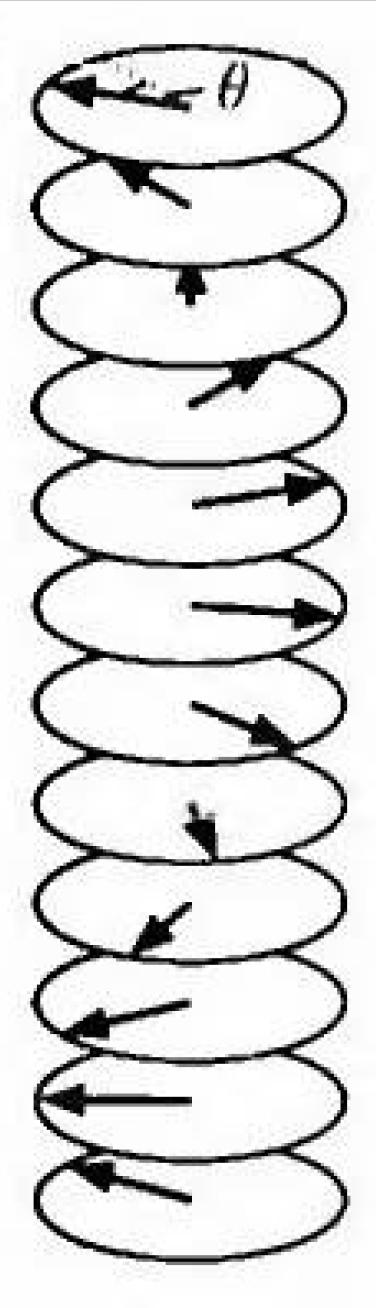
\includegraphics[scale=0.3]{05-Helical.png}
    %\label{Fig:05-04-01}
\end{wrapfigure}

En muchas tierras raras la estructura cristalino se dispone en capas. Consideremos entonces que la interacción entre capas puede describirse usando la constante de permutación respecto los vecinos mas cercanos $\Jsf_1$ y la de los siguientes mas cercanos $\Jsf_2$. Si el ángulo entre cada uno de los momentos magnéticos es $\theta$, siendo este constante entre cada uno de los planos, tendremos que si hay $N$  planos con espines $S$, el valor de la energía

\begin{equation}
    E =  \sum_i^N \sum_{\delta=-2}^2 \Jsf_{ij} \Sn_{i} \cdot \Sn_{i+\delta} =- 2 N S^2  (\Jsf_1 \cos (\theta) + \Jsf_2 \cos (2 \theta))
\end{equation}
donde es importante recordar que cada plano tiene dos vecinos cercanos, uno por arriba y otro por abajo. Queremos ver cuando la energía es minima. Para esto debemos derivar e igualar a cero. Así:

\begin{equation}
    (\Jsf_1 + 4 \Jsf_2\cos (\theta)) \sin \theta = 0
\end{equation}
de tal modo que existen 2 soluciones: una que anule el seno y otra que anule el paréntesis. Para anular el seno, tendríamos dos posibilidades, $\theta=0$ o $\theta=\pi$. El primero implica que los momentos magnéticos de los planos son paralelos y por tanto estamos ante \textit{ferromagnetismo}. La segunda implica que los momentos son antiparalelos y por tanto estamos ante \textit{antiferromagnetismo}. La otra posiblidad es que

\begin{equation}
    \cos (\theta) = - \frac{\Jsf_1}{4 \Jsf_2}
\end{equation}
Esta solución corresponde al \textbf{ordenamiento helimagnético}, también llamado \textbf{helimagnetismo}. Si $\Jsf_1<0$, tendremos que para los valores de $\Jsf_1/4 > \Jsf_2$ tendrá menos costo energético tener una estructura helimangnética, al igual que si $\Jsf_1>0$ para los valores $-\Jsf_1>\Jsf_2$. En función de la región del plano $\Jsf$ que nos encontremos hallaremos una estrucutura u otra.  

%\section{Spin glasses}

%\section{Ordenamiento nuclear}

%\section{Medidas del ordenamiento magnético}

\newpage

\chapter{Simetría, orden y su rotura}

La aparición de un orden espontáneo a bajas temperaturas es fundamental para entender la materia condensada. Tanto materiales ferromagnéticos, como materiales antiferromangéticos, líquidos cristalinos y superconductores son fases \footnote{del ingles \textit{phases}} (estados de la materia) con un cierto grado de orden. Todos estos fenómenos comparten propiedades fundamentales, como puede ser la aparición de una \textbf{temperatura crítica} $T_C$, que diferencia las propiedades físicas en dos regiones térmicas. Por encima de esta temperatura crítica se puede considerar que el ordenamiento desaparece. Debe entonces existir algún tipo de parámetro que nos de una medida del orden del sistema, tal que sea nulo cuando $T>T_C$ y no nulo cuando $T<T_C$. Por ejemplo para el ferromagnetismo la magnetización es un parámetro de orden, y para el antiferromagnetismo es $M_+-M_-$. En este capítulo trataremos entonces cada uno de los tipos de parámetros de orden asociados a la rotura de la simetría. Primero hablaremos un poco de la simetría.

\section{Simetría}

Se dice que un sistema posee \textbf{simetría} si el Hamiltoniano que la describe es invariante frente a una trasformación asociada a un grupo de simetría. Un grupo de simetría es una colección de elementos u operaciones (ej: cambios de variables), que siguen una serie de relgas. La regla principal es que el grupo debe ser cerrado: una combinación de dichos elementos/operaciones debe pertenecer también al grupo. Otras reglas son: la combinación debe ser asociativa, invertible y bien definida. \\

Hablamos de \textbf{simetría discreta} si en el grupo existe un número contable de elementos, como puede ser la simetría esférica de un cubo.  La \textbf{simetría continua} contiene un número no contable de elementos continuos, como puede ser la simetría esférica de una esfera. Decimos que el sistema posee \textbf{simetría global} si es invariante en todos los puntos del espacio bajo dicha transformación. Si depende del punto del espacio diremos qeu el sistema posee \textbf{simetría local}. Por ejemplo la simetría de gauge de un superconductor es una simetría local. \\


Para entender el concepto de rotura espontánea de simetría hace falta hacer algún tipo de analogía con algún otro fenóeno físico, no en pos de relacionar los modelos o crear un isomorfismo, si no de entender el concepto. El ejemplo más útil no es ninguno proveniente del estado sólido. Supongamos un tubo de plástico o madera. En un principio se encuentra ordenada, con una simetría de tipo cilíndrico. Si colocamos en la parte superior de la misma un peso bajo, el tubo no sufrirá ninguna modificación: seguirá teniendo su simetría. Sin embargo si continuamos colocando masa encima, existirá un punto, un peso a partir del cual el tubo comenzará a doblarse, o incluso a romperse. Por supuesto esto dependerá del material. En cualquier caso se habrá roto la simetría del sistema, el tubo ya no será simétrico. De hecho será imposible (o tendrá un costo energético muy elevado) recomponer el tubo. En este caso la rotura de la simetría cilíndrica ha collevado a un cambio físico empírico, medible. Esto mismo también ocurre con los el cambio de estado líquido-sólido. Un líquido presenta simetría esférica porque todas las partículas están en posiciones completamente distintas. Sin embargo existe una temperatura a partir la cuál el líquido se convierte en sólido, donde existe un orden que rompe la simetría. Al ordenarse en una determinada dirección, el sólido (por ejemplo de hielo) ya no será invariante al rotarlo. \\

Esto precisamente ocurre con los materiales ferromagnéticos. Un material ferromagnético por debajo de una temperatura (la temperatura de Curie) estará completamente ordenado: todos los momentos magnéticos apuntan en la misma dirección. Sin embargo es este mismo orden el que hace que no haya simetría. Cuando el material está en su estado paramagnético, debido a que cada uno de los momentos apuntan en una dirección aleatoria, y por tanto no existe una dirección neta preferencial por la magnetización, tiene una simetría esférica (al menos localmente). \
 

\section{Modelos} \label{Sec:06-02}

Para debatir sobre las consecuencias de la rotura espontánea de simetría es conveniente crear algunos modelos simples sobre el magnetismo. 

\subsection{Teoría de Landau sobre el ferromagnetismo} \label{Subsec:06-02-01}

Un modelo interesante es el modelo creado por el físico ruso Lev Landau. Este modelo comienza creando una energía libre de Helmholtz $F$ con dependencias cuadráticas respecto la magnetización, tal que

\begin{equation}
    F(M) = F_0 + a(T) M^2 + bM^4
\end{equation}
donde $F_0$ y $b$ son constantes ($b>0$) y $a(T)$ una función de la temperatura. Se puede demostrar que existe una transición de fase si permitimos que $a(T)$ tenga un cambio de signo para la temperatura $T_C$. Esto es equivalente a decir que cerca de $T_C$ su forma es $a(T)=a(T-T_C)$ donde $a_0>0$. De nuevo queremos encontrar el estado fundamental, esto es, la magnetización para la cual la energía se minimiza. Haciendo $\partial F / \partial M = 0 $, tenemos que este viene dado por:

\begin{equation}
    M=0 \tquad M = \pm \ccorchetes{\frac{a_0 (T_C-T)}{2b}}^{1/2}
\end{equation}

\begin{figure}[h!]
    \centering
    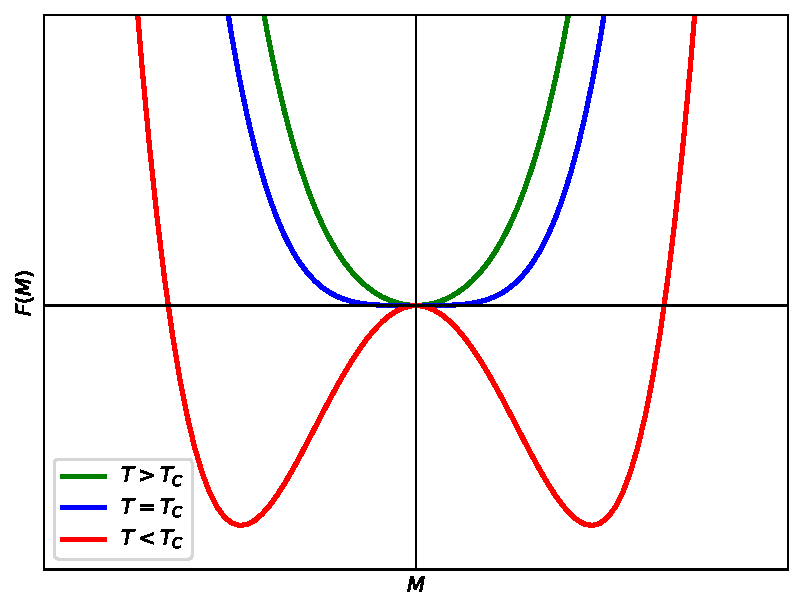
\includegraphics[scale=0.8]{06-Landau.pdf}
    \caption{la energía libre en función de $M$ para algunas temperaturas.}
    \label{Fig:06-02-01}
\end{figure}

La segunda condición es válida únicamente si $T<T_C$ (lo cual es evidente, pero no por ello ignorable). Podemos ver que por encima de $T>T_C$ el estado fundamental es unívoco. Sin embargo para temperaturas inferiores tendremos que existen dos posibles estados de equilibrio, uno con $M$ positiva y otro con $M$ negativa. Esto se puede ver perfectamente en la figura \ref{Fig:06-02-01} . \\

La forma de estudiar las transiciones usando el modelo de Landau se llama \textbf{teoría del campo medio}, aunque se puede llamar de manera jocosa el estudio a ``la Landau''. La razón por la cuál se llama así es que se asume que todos los espines de un cuerpo sufren de manera igual el mismo campo, el campo medio neto de los vecinos. En general las teorías de campo medio son las teorías mas simples que se pueden hacer para tratar de describir los diferentes tipos de transición. Aunque en función de su aplicación tengan diferentes nombres, la base es la misma. Es muy importante mencionar que la teoría de campo medio ignora completamente las fluctuaciones, las cuales son muy fuertes cerca de la zona de transición. Es de esperar entonces que cerca de la región de transición esta teoría falle. 

\subsection{Modelo de Heisenberg y de Ising}

Otra manera alternativa de estudiar el comportamiento magnético de los sólidos es consdierar los modelos microscópicos particulares de las interacciones magnéticas. El \textbf{modelo de Heisenberg} (ecuación \ref{Ec:02-03-004})nos relaciona la influencia sobre el espín $i$ de los átomos vecinos $j$. Por completitud escribimos aquí su ecuación:


\begin{equation}
    \Hcal = - \sum_{(i,j\rangle} \Jsf_{ij} \Sn_i \cdot \Sn_j 
\end{equation}
Un modelo similar es el \textbf{modelo de Ising}, que viene dado por:

\begin{equation}
    \Hcal = - \sum_{(i,j\rangle} \Jsf S_i^z S_j^z 
\end{equation}
Es muy imporatnte distinguir entre la \textit{dimensionalidad de la red}  $d$ en la cuál se encuentran los espines y la \textit{dimensionalidad de los espines} $D$ (a $D$ también se le llama \textit{parámetro de orden}). Por ejemplo para el modelo de Heisenberg $D=3$ (los espines son vectores), y en el modelo de Isint $D=1$ al considerar solo su parte en la dirección $\hnz$. Sin embargo podemos considerar redes de $d=1,2,3,4...$ dimensiones para ambos modelos.

\section{Consecuencias de la rotura de simetría}

Cuando tu rompes la simetría existen varias consecuencias: \\

\begin{itemize}
    \item \textbf{Transiciones de fase:} el sistema tendrá un cambio de comportamiento (cambio de las propiedades) a la temperatura $T_C$. La región cercana a la transición de fase se llama la \textbf{región crítica}. \\
    
    \item \textbf{Rigidez:} una vez la simetría está rota \footnote{del ingles \textit{having broken the simmetry}.} (una vez ya no hay simetría) habrá que invertir mucha energía para devolver la simetría al sistema. Por esa misma razón los cristales no se rompen fácilmente, y los materiales ferromagnéticos muestran magnetismo permanente.  \\

    \item \textbf{Excitaciones:} en el cero absoluto ($T=0$) el sistmea está perfectamente ordenado. Para una temperatura finita el orden se hace más débil debido a las posibles excitaciones en el parámetro de orden. Dichas excitaciones tienen un nombre: en el caso de los cristales se les llama \textit{ondas reticulares} cuantizadas en los \textit{fonones}, en el caso de los materiales ferromagnéticos se les llama \textit{ondas de espín} cuantizadas en los \textit{magnones}. \\

    \item \textbf{Defectos:} si la simetría se ha roto de manera diferente en dos partes espacialmente diferenciadas del material, tendremos que en la frontera de las mismas habrá un defecto. En el caso de los cristales tendremos las \textit{deslocalizaciones}, en el caso de los ferromangéticos tendremos las \textit{paredes de dominio}.    
\end{itemize}

\section{Transiciones de fase}

En el apartado \ref{Subsec:06-02-01} hemos presentado la teoría ferromagnética de Landau. En esta teoría llegamos a que la magnetización se comporta como $M\varpropto (T_C-T)^{1/2}$ (por debajo de la temperatura crítica). Experimentalmente el comportamiento es del tipo $(T_C-T)^{\beta}$ (cerca de la transición). El exponente $\beta$ nos da una información muy importante acerca de la naturaleza de la transición de fase. Un número finito de otros exponentes, que llamaremos \textbf{exponentes críticos}, pueden ser definidos, conteniendo información muy interesanet acerca de la transición de fase. En la región crítica se ha hallado, experimentalmente, que

\begin{equation}
    \begin{array}{lllll}
       \chi & \varpropto  & (T-T_C)^{-\gamma} & \tquad & T > T_C   \\
       M & \varpropto  & (T_C-T)^{\beta} & \tquad &  T < T_C   \\
       M & \varpropto  & H^{1/\delta} & \tquad & T = C   \\
    \end{array}
\end{equation}
donde $\beta, \gamma$ y $\delta$ son los \textit{exponentes críticos}. \\

\begin{table}[h!]
    \centering
    \begin{tabular}{ccccc}\hline
       \textbf{Modelo}  & \textbf{Campo medio} & \textbf{Ising} & \textbf{Ising} & \textbf{Heisenberg}  \\ \hline
       $D$  & cualquiera & 1 & 1 & 3 \\
       $d$  &  cualquiera  & 2 & 3 & 3 \\
       $\beta$  &  1/2 & 1/8 & 0.326 & 0.367 \\
       $\gamma$  &  1 & 7/4 & 1.2378 & 1.388 \\
       $\delta$  &  3 & 15 & 4.78 & 4.78 \\
         \hline
    \end{tabular}
    \caption{Exponentes críticos para diferentes modelos}
    \label{Tab:06-04-01}
\end{table}
Como hemos dicho antes, las fluctuaciones son ignoradas por las teorías de campo medio. Esto implica que no son buenas describiendo las cercanías de $T_C$. Sin embargo si son buenas prediciendo los sistemas con $d\geq4$, prediciendo correctamente sus exponentes críticos. Debido al desastre que supone que nuestra teoría no sea capaz de predecir correctamente comportamientos con $d\leq4$, necesitamos algun modelo ideal estadístico que nos permita calcular dichos parámetros. Las transiciones de fase, experimentalmente, no depende del tipo de transición que sea (si es gas-líquido, ferromagnética-paramagnética...) solo parece depender únicamente de los siguientes factores:\\

\begin{itemize}
    \item La dimensionalidad del sistema $d$.
    \item La dimensionalidad del parámetro de orden $D$.
    \item Si las fuerzas son de corto o largo alcance.\\
\end{itemize}
Por tanto basta con encontrar cual es el mejor método para los valores partículares de $D$ y $d$ (así como el tipo de fuerza). Los métodos que tenemos ahora son los siguientes:\\

\begin{itemize}
    \item Para los casos $d=1$ los sistemas no suelen presentar transiciones de fase continuas.
    \item Para los casos $d\geq4$ usamos las teorías de campo medio. 
    \item Para los casos de fuerzas de largo alcance usamos la teoría de campo medio. 
    \item Para el caso de $d=2,D=1$ usamos el modelo de Ising 2D. 
    \item Para el caso $D=\infty$ usamos el llamado \textit{modelo esférico}. \\
\end{itemize}

Desafortunadamente, la mayoría de las situaciones reales corresponden a $d=3$ y fuerzas de corto alcance, las cuales no se han resuelto todavía. 


\section{Rigidez}

Romper la simetría conlleva elegir uno estado fundamental partícular: ¿Hacía donde apuntan los espines?¿Arriba, abajo, a la izquierda...? La energía es minimizada cuando la simetría es rota en todos las partes por igual (no hay ningún defecto). Si tu tratas de cambiar levemente partes del material (rompiendo la simetría de manera diferente), aparecerán fuerzas que repercutirán en un mayor energía en el sistema. Esta energía necesaria para poder cambiar partes del sistema se reflejará en la \textbf{rigidez} del material. Por esta misma razón los cristales no se deforman fácilmente: se necesita una energía elevada para mover parte de la estructura cristalina un mínimo. Estas ideas aplicadas al ferromagnetismo permietn explicar el fenómeno del \textbf{magnetismo permanente} de algunos materiales. Una vez los espines están alineados en una dirección, hacer que cambien de dirección costará bastante energía (siendo esta energía proprocional a $(\nabla M)^2$ en el caso de magnetización no-uniforme).

\section{Excitaciones}

Un solido a temperatura $T=0$ está completamente ordenado. A una temperatura no nula, aparecerán vibraciones de red en el caso de los cristales (esto es, los átomos comenzarán a vibrar en su posición de la red cristalina), las cuales estarán cuantizadas en los \textbf{fononoes}. Los fonones estarán caracterizados por una \textbf{relación de dispersión}, la cual relacionará la frecuencia angular y el vector de onda ($\omega$ y $q$ respectivamente). En el caso de los materiales ferromagnéticos un fenómeno similar ocurrirá: a una temperatura $T=0$ todos los espines están perfectamente orientados y ordenados, apuntando en la misma dirección. Si aumentamos la temperatura, aparecerán vibraciones en el seno de los espines, vibraciones en su dirección, que llamaremos \textbf{ondas de espín}, que cuantizaremos en los \textbf{magnones}.  

\subsection{Magnones}

Supongamos un material ferromangético isótropo, que verificará el modelo de Heisenberg, a dos vecinos. Tendremos dos maneras de resolver el problema de las ondas de espín, la primera es usar la aproximación semiclásica, y la segunda usando directametne la mecánica cuántica. En ambas llegaremos al mismo resultado. El modelo de Heisenberg usado es, entonces:

\begin{equation}
    \Hcal = - 2 \Jsf \sum_i \Sn_i \cdot \Sn_{i+1}
\end{equation}

\subsubsection{Aproximación semiclásica}

Según el teoréma de Ehrenfest, tendemos que la evolución temporal del espín $\Sn_j$ (el espín de una posición \textit{cualquiera}) vendrá dado por:

\begin{equation}\begin{array}{lll}
    \dfrac{\D \langle \Sn_j \rangle}{\D t}  & = & \dfrac{1}{i \hbar} \langle \ccorchetes{\Sn_j , \Hcal} \rangle  \\ \\ & = & - \dfrac{2\Jsf}{i \hbar} \langle \ccorchetes{\Sn_j,\Sn_j \cdot \Sn_{j-1}} + \ccorchetes{\Sn_j, \Sn_j \cdot \Sn_{j+1}} \rangle \\ \\
     & = &  - \dfrac{2\Jsf}{i \hbar} \langle \Sn_j \times (\Sn_{j-1}+ \Sn_{j+1} \rangle \\
\end{array}
\end{equation}
Ahora si tratamos los espines como vectores clásicos (del tratamiento inicial cuántico pasamos al tratamiento clásico), de tal manera que podamos considerar que todos los espines están alineados entorno al eje z $S_j^z = S$. Entonces si consideramos un desplazamiento leve, una mínuscula perturbación, tal que $S_j^x,S_j^y \ll S_j^z$, tendremos la siguientes ecuaciones:

\begin{equation}
    \derivadas{S^x_j}{t} \approx \frac{2JS}{\hbar} \parentesis{2S_j^y-S_{j-1}^y-S_{j+1}^y}
\end{equation}
\begin{equation}
    \derivadas{S^y_j}{t} \approx \frac{2JS}{\hbar} \parentesis{2S_j^x-S_{j-1}^x-S_{j+1}^x}
\end{equation}
\begin{equation}
    \derivadas{S^z_j}{t} \approx 0 \label{Ec:06-06-05}
\end{equation}
Como podemos ver hemos despreciado completamente todos los términos que van con $(S^x)^2,(S^y)^2,(S^xS^y)$. Por esta mismar razón se verifica la ecuación \ref{Ec:06-06-05}. De este modo las soluciones vendrán dadas por:

\begin{equation}
    S_j^x = A e^{i(qja-\omega t)} \tquad S_j^y = B e^{i qja-\omega t}
\end{equation}
donde $A=iB$ (esto se debe a que las ecuaciones están acopladas). Se puede demostrar también que se verifica la relación de

\begin{equation}
    \hbar \omega = 4 \Jsf S (1- \cos (qa))
\end{equation}
Esta es la \textit{relación de dispersión} para las ondas de espín. En la figura siguiente traemos una imagen de los diferentes espines rotando alrededor del eje $z$, y como en función de la posición cambian. Por cuestiones obvias en la imagen no se verifica $S^x,S^y \ll S^z$. \\


\subsubsection{Metodo cuántico}
Consideremos el estado fundamental del sistema $\Phi$, donde todos los espines están alineados en la direción $+z$. En una dimensión el hamiltoniano del modelo de Heisenberg consistirá en:
\begin{equation}
    \Hcal = - 2\Jsf \sum_i \ccorchetes{S_i^z S_{i+1}^z + \frac{1}{2} \parentesis{S_i^+ S_{i+1}^- + S_i^- S_{i+1}^+}}
\end{equation}
de tal modo que $\Hcal  |\Phi\rangle=-NS^2\Jsf |\Phi\rangle$. Supongamos una excitación, un espín que se ha girado (\textit{flipped} en inglés) en el sitio $j$. Llamaremos al estado $|j\rangle$ al estado en el cuál al espín $j$ le han dado la vuelta, tal que $|j\rangle = S_j^- |\Phi\rangle$. Virar un espín implica que hemos cambiado el espín total por $1/2-(-1/2)$, esto es, uno. Esta excitación tiene un espín de tamaño unidad, y por tanto es un bosón. A este bosón se le llamará \textbf{magnón}. Si aplicamos el hamiltoniano a este estado tendremos que
\begin{equation}
    \Hcal |j\rangle = 2 \ccorchetes{(-NS^2\Jsf+2S\Jsf)|j\rangle - S\Jsf |j+1\rangle - S\Jsf|j-1\rangle}
\end{equation} 
de tal modo que $|j\rangle$ no es un autoestado. Un autoestado es $|q\rangle$ tal que

\begin{equation}
    |q\rangle = \frac{1}{N} \sum_j e^{i q R_j} |j\rangle
\end{equation}

que no es el estado de espín invertido deslocalizado. Aplicandole el hamiltoniano:
\begin{equation} 
    \Hcal |q\rangle = E(q) |q\rangle 
\end{equation}
de tal modo que
\begin{equation}
    E(q) = - 2 NS^2 \Jsf + 4 \Jsf S (1- \cos (qa)) \label{Ec:06-06-12}
\end{equation}
y usando la relación de Plank $\hbar \omega = E(q)$, llegaremos a la misma relación de dispersión que en la aproximación semiclásica. 

\begin{figure}[h!]
\centering
\begin{tikzpicture}

\filldraw[ultra thick,fill=black!4] (0,0) ellipse (1.2 and 0.6);
\draw[arrows={->},ultra thick] (0,-3) -- (1.2,0);
\draw[thick] (0,-3) -> (0,0);


\filldraw[ultra thick,fill=black!4] (3,0) ellipse (1.2 and 0.6);
\draw[arrows={->},ultra thick] (3,-3) -- (4,0.3);
\draw[thick] (3,-3) -- (3,0);


\filldraw[ultra thick,fill=black!4] (6,0) ellipse (1.2 and 0.6);
\draw[arrows={->},ultra thick] (6,-3) -- (6.8,0.48);
\draw[thick] (6,-3) -- (6,0);


\filldraw[ultra thick,fill=black!4] (9,0) ellipse (1.2 and 0.6);
\draw[arrows={->},ultra thick] (9,-3) -- (9.2,0.56);
\draw[thick] (9,-3) -- (9,0);


\filldraw[ultra thick,fill=black!4] (12,0) ellipse (1.2 and 0.6);
\draw[arrows={->},ultra thick] (12,-3) -- (11.7,0.55);
\draw[thick] (12,-3) -- (12,0);

\end{tikzpicture}
\caption{ondas de espín a travñes de espines linealmente orientados}
\label{Fig:06-06-01}
\end{figure}

\subsection{Dependencia antiferromagnética}

Como hemos visto la dependencia ferromagnética va con un coseno. Si consideramos la energía $E_0$ que tendría en el estado fundamental, la relación de dispersión vendrá dada por:

\begin{equation}
    \hbar \omega = E_0 + 4 \Jsf S (1-\cos (qa))
\end{equation}
La pregunta que nos hacemos es: ¿Cuál será la dependencia de un antiferroimán? Como todo lo que sucedeen los antiferromagnéticos, el cálculo va a resultar mucho mas complicado. En un primer lugar habría que considerar que en función de si $i$ es par/impar el espín estará hacia $\uparrow/\downarrow$, por lo que tendremos diferentes ecuaciones de evolución temporal. El cálculo lo dejamos como ejercicio, siendo el resultado final el siguiente:

\begin{equation}
    \hbar \omega = E_0 + 4 \Jsf S \sin (qa)
\end{equation}
Cuando $q \rightarrow 0$ podemos ver que las exticaciones mangéticas de un ferroimán serían cuadráticas $\cos(qa)\sim 1 +(qa)^2$, mientras que las de un antiferroimán serían lineales $\sin(qa) \sim qa$. 

\subsection{La ley de Bloch $T^{3/2}$}

Para campos pequeños, tal que $\cos (qa) \approx 1 - \frac{(qa)^2}{2}$. Consecuentemente la ecuación \ref{Ec:06-06-12} queda de la forma

\begin{equation}
    \hbar \omega \approx 2 \Jsf q^2 a^2
\end{equation}
Tenemos que hallar la ecuación de densidad de estados. Para un oscialdor armínico en 3 dimensiones $g(q) \varpropto q^2$, $g(\omega) = \omega^{1/2}$. Como hemos dicho, las ondas de espín se pueden cuantizar en \textbf{magnones}, que son bosones (espín $1$). El número de modos de las posibles exitaciones a la temperatura $T$ la denotaremos por $n_{\mathrm{magnon}}$, y se puede calcular como:

\begin{equation}
    n_{\mathrm{magnon}} = \int_0^\infty \frac{g(\omega) \D \omega}{\exp (\hbar \omega /k_B T) - 1} \label{Ec:06-06-14}
\end{equation}
donde al factor del denominador se le conoce como el \textit{factor de Bose} (que es fundamental para estudiar los gases cuánticos de bosones, dados por la mecánica de Bose-Einstein). Si $g(\omega) \varpropto \omega^{1/2}$ (aproximación a bajas temperaturas), y hacemos el cambio $x=\hbar \omega/k_B T$, tenemos que:

\begin{equation}
    n_{\mathrm{magnon}} = \parentesis{\frac{k_B T}{\hbar}}^{3/2} \int_0^\infty \frac{x^{1/2} \D x}{\exp (x) - 1} \varpropto T^{3/2} \label{Ec:06-06-15}
\end{equation}
dado que cada modo de exitación (en inglés \textit{magnon mode}) reduce la magnetización total (porque cada magnon es un estado deslocalizado de espín invertido), tendremos que a una temperatura baja se verifica que

\begin{equation}
    \frac{M(0)-M(T)}{M(0)} \varpropto T^{3/2}
\end{equation}
Este resultado es denominado como la \textbf{ley de Bloch} $T^{3/2}$. No solo es un resultado interesante desde el punto de vista teórico, si no que además es capaz de predecir con precisión los datos experimentales para un regimen a baja temperatura. La energía de un modo de magnón viene dada por:

\begin{equation}
    E_{\mathrm{magnon}} = \int_0^\infty \frac{\hbar \omega g(\omega) \D \omega}{\exp(\hbar \omega / k_B T)-1}
\end{equation}
por lo que la capacidad calorífica $C=\partial E_{\mathrm{magnon}} / \partial T$ es proporcional a $T^{3/2}$.

\subsection{Teorema de Mermin-Wagner-Berezinski}

En dos dimensiones la integral \ref{Ec:06-06-14} diverge, por lo que $M \rightarrow 0$ para todo $T>0$ para un modelo de Heisenberg isótropo en 1-D y 2-D. El número total de ondas de espín que es generada por una temperatura finita diverge, y por tanto el ferromagnetismo espotáneo no debería ser posible. Este resultado fue demostrado independientemente por Berezinski y por Mermin y Wagner, y condensado en el \textbf{teorema de Mermin-Wagner-Berezinski}, que establece que las simetrías continuas no pueden ser rotas espontáneamente a temperatura finita en sistemas con interacciones de corto alcance en dimensiones $d\leq 2$. \\

Este resultado solo aplica a los materiales ferromangéticos isótropos que sigan el modelo de Heisenberg. En el caso de que el material presente algún tipo de anisotropía, no debería verificarse. Un material con isotropía posee una simetría rotacional que nos permite cambiar la dirección global de los espines sin costo alguno de energía. Entonces las ondas de espín con grandes longitudes de ondas (en este tipo de ondas las interacciones ocurren entre átomos a mucha distancia) cuestan una energía muy pequeña. Al ser tan poco energéticas, las fluctuaciones son capaces de destruir las interacciones de largo alcance, evitando así fenómenos como el ferromagnetismo. \\

Dado que la energía anisótropoa crece con el cuadrado de la distancia, tendremos que la propia anisotropía cancela estas flucutaciones. Es la rotura de simetría las que permite que las interacciones de largo alcance se estabilicen. Otra fuente de anisotropía puede ser la interacción dipolar entre espines (más debil que la interacción de intercambio), que puede actuar del mismo modo, suprimiendo las fluctuaciones.  


\section{Dominios}

En las diferentes regiones del sistema macroscópico la simetría se rompe de maneras diferentes. Entonces en la superficie de separación entre estas regiones puede romperse la rigidez. A estas superficies, en el caso de materiales ferromagnéticos, las llamaremos \textbf{paredes de dominio}. \\

Weiss fue el primero en proponer que un material ferromagnético presenta regiones llamadas \textbf{dominios}, en los cuales la magnetización local alcanza la de saturación, pero apunta en una dirección no necesariamente idéntica a la de los otros dominios. La existencia de los dominos explica el hecho soprendente de que algunos materiales ferromagnéticos (llamados \textit{suaves}) alcancen la magnetización de saturación al aplicarle campos magnéticos pequeños. La razón es evidente: los campos magnéticos ya están ordenados, por lo que un pequeño campo magnético que los haga paralelos será suficiente para alcanzar la magnetización de saturación, y, sin embargo, bajo un campo magnético aplicado nulo la magnetización neta será nula, ya que cada domimio apuntará a un sitio diferente. 


\subsection{Parades de dominio}

Entre dos dominios adyacentes existe una superficie de separación llamada pared de domino. Las paredes de dominio se pueden clasificar en función del ángulo entre estas y la magnetización de dos dominios. En la figura \ref{Fig:06-07-01-a} puede verse una pared de dominio a 180º, que implica que ambas magnetizaciones tienen un ángulo entre sí de 180º; y en la figura \ref{Fig:06-07-01-b} puede verse una pared de dominio a 90º, que implica que ambas magnetizaciones tienen un ángulo entre sí de 90º. \\

Para un material ferromagnético rotar un espin cuesta energía (debido al espín de los vecinos). Como sabemos dos espines presentan la siguiente energía $-2\Jsf \Sn_1\cdot \Sn_2=-2\Jsf S^2 \cos (\theta)$. Si el ángulo es pequeño ($\theta \ll 1$), tendremos que la diferencia de energía vendrá dada por $\Jsf S^2 \theta^2$ (con $\theta \ll 1$, para poder hacer $\cos (\theta) \approx 1 + \theta^2/2$). \\

Llamamos pared de Bloch a un tipo de pared donde cada espín gira un ángulo $\theta<<1$ respecto al anterior, en una línnea recta. Supongamos entonces esta línea formada por $N$ espines tal que del primer al último hay un desfase total de $\pi$, de tal modo que $\theta = \pi /N$, y por tanto la contribución será $\Jsf S^2 \pi^2/N$. Para calcular la energía por unidad de superficie $\sigma_{BW}$ (que es el costo energético que nos interesa) de este tipo de pared usaremos que en una pared de $1m^2$ hay $1/a^2$ líneas de espín, de tal modo que

\begin{equation}
    \sigma_{BW} = \Jsf S^2 \frac{\pi^2}{Na^2}
\end{equation}
que, lógicamente, tiende a cero si $N\rightarrow\infty$. 


\begin{figure}[h!] \centering
\begin{subfigure}[b]{0.45\linewidth} \centering
\begin{tikzpicture} 
\filldraw[thick,fill=black!5] (-1.5,0) rectangle (1.5,3);
\draw[arrows={->},ultra thick] (-0.75,0.5)--(-0.75,2.5)  ;
\filldraw[thick,fill=black!15]  rectangle (1.5,3);
\draw[arrows={->},ultra thick] (0.75,2.5)--(0.75,0.5)   ;
\end{tikzpicture}
\caption{dominio 180º.}
\label{Fig:06-07-01-a}
\end{subfigure}
\begin{subfigure}[b]{0.45\linewidth} \centering
\begin{tikzpicture}
\filldraw[thick,fill=black!5] (0,0) -- (3,3) -- (0,3) -- cycle;
\draw[arrows={->},ultra thick] (0.2,2.5)--(1.8,2.5)  ;
\filldraw[thick,fill=black!15] (0,0) -- (3,3) -- (3,0) -- cycle;
\draw[arrows={->},ultra thick] (2.5,1.5)--(2.5,0.2) ;
\end{tikzpicture}
\caption{dominio 90º}
\label{Fig:06-07-01-b}
\end{subfigure}
\caption{Clasificación paredes dominio.}
\end{figure}

\subsection{Anisotropía magnetocristalina}

Los cristales poseen \textbf{ejes magnéticos duros} y \textbf{ejes magnéticos suaves}. Esto hace que para ciertas direcciones el crital sea más sencillode magnetizar que otras direcciones. La energía para un cristal cúbico la expresión de la energía:

\begin{equation}
    E = K_1 (m_x^2 m_y^2 + m_y^2 m_z^2 + m_z^2 m_x^2) + K_2 m_x^2 m_y^2 m_z^2 + \cdots
\end{equation}
donde $\mn =(m_x,m_y,m_z)=\Mn / | M |$. En coordenadas esféricas:

\begin{equation}
    E = K_1 \parentesis{\frac{1}{4}\sin^2(\theta) \sin^2(2 \phi) + \cos ^2 (\theta) } \sin^2(\theta) + \frac{K_2}{16} \sin^2(2 \phi) \sin^2(2\theta) \sin^2(\theta) + \cdots
\end{equation}
Esta anistotropía puede explicarse usando la interacción espín-órbita y la extinción parcial del momento angular orbital. Un término adicional es debido a la desimanación, asociada a la forma del material. A este término se le llama \textbf{anistropía geométrica}. En láminas delgadas suele ser $\frac{1}{2} \mu_0 M^2 \cos^2(\theta)$, siendo $\theta$ el ángulo entre la normal a la superficie y $\Mn$. Una de las formas mas simples que puede tener el término energético anisótropo viene dado por

\begin{equation}
    E=K_1 \sin^2(\theta) + K_2 \sin^4 (\theta)
\end{equation}
y es el término asociado a materiales donde formados por planos concatenados, de tal manera que $\theta$ es el ángulo entre dichos planos y la magnetización.

\subsection{Grosor de la pared de dominio}

En los dominios de un material ferromagnétio, la magnetización prefiere ir en la dirección del eje suave, pero entre dominios, en una pared de dominio, esta va a girar, por lo que habrá una componente que vaya por el eje duro, con un incremento del costo energético. Asumiendo el término más sencillo posible para el término anisótropo $E=K \sin^2(\theta)$ donde $K$ es la constante anisótropa, podremos hacer una aproximación del costo energético de una pared de Bloch. Si llevamos al continuo el término, tal que

\begin{equation}
    \sum_{i=1}^K K \sin^2(\theta_i) \approx \frac{N}{\pi} \int_0^\pi K\sin^2(\theta) = \frac{NK}{2}
\end{equation}
podemos ver que la energía por unidad de área vendrá dada por $NKa/2$. En ese caso la energía total:

\begin{equation}
    \sigma_{BW} = \Jsf S^2\frac{\pi^2}{Na^2} + \frac{NKa}{2}
\end{equation}
por lo que ahora no se va a cero cuando $N\rightarrow\infty$. Por esa misma razón no vemos paredes de dominio (de Bloch) infinitas. La ecuación de equilibrio se alcanzará cuando se verifique  $\D E_{BW} / \D N$, o lo que es lo mismo:

\begin{equation}
N = \pi S \sqrt{2 \Jsf / K a^3}
\end{equation}
por lo que el grosor de la pared de Bloch vendrá dado por

\begin{equation}
    \delta = NA=\pi S\sqrt{\frac{2\Jsf}{Ka}}
\end{equation}
donde $a$ es la distancia entre átomos, también llamado espacio de red (del inglés \textit{lattice spacing}). Un término de $\Jsf$ grande hace que la pared sea mas gruesa, y un término de $K$ mas grande hace que sea mas fina. La energía por unidad de área del dominio en esta configuración:

\begin{equation}
    \sigma_{BW} = \pi S\sqrt{\frac{2 \Jsf K}{a}}
\end{equation}

\subsection{Formación de los dominios}

Dado que las paredes de dominio tienen un costo energético, sería sensato plantearse que cómo se forman los dominios. La razón de la formación de dominios se puede hacer desde la magnetostática, y es que reduce la energía asociada a los términos dipolares magnéticos. Sabemos que la energía de un sistema magnético:

\begin{equation}
    E = \frac{\mu_0}{2} \int \Hn^2  \D V \label{Ec:06-07-10}
\end{equation} 
usando la ecuación característica $\Hn = \mu_0 \Bn - \Mn$, y que el término $\int \Bn \cdot \Hn \ \D V=0$ (resultado que se deduce de las ecuaciones de Maxwell $\nabla \cdot \Bn = 0$ y $\nabla \times \Hn = 0$), podemos la ecuación \ref{Ec:06-07-10} en 

\begin{equation}
    E = - \frac{\mu_0}{2} \int \Mn \cdot \Hn \ \D V
\end{equation}
Si el campo $\Hn$ es el campo desimanador $\Hn_d$ (que depende de la geometría del material, y verifica que $\Hn \varpropto - \Mn$), tenemos la expresión de la \textbf{energía de desimanación}, dada por

\begin{equation}
    E = - \frac{\mu_0}{2} \int \Mn \cdot \Hn_d \ \D V
\end{equation}
y por tanto la energía vendrá dada por

\begin{equation}
    E =\frac{\mu_0}{2} N M^2 V
\end{equation}
donde $N$ es el \textbf{factor desimanador} (en una esfera $N=1/3$). Ahora bien: ¿Por qué la aparición de dominios reduce dicho término energético? La razón de esto es que al aparecer paredes, donde las condiciones de frontera cambian, el factor desimanador se reduce. Sin embargo la cantidad de dominios que aparecen tiene un límtie impuesto, precisamente, por el costo energético que estos tienen. Por eso existe un \textit{número de dominios finito}. 

\begin{figure}[h!] \centering
\begin{subfigure}{0.45\linewidth} \centering
\begin{tikzpicture}[thick,scale=0.6]
\filldraw[fill=black!15] (0,0)  rectangle (3.2,5);
\draw[arrows={->},ultra thick] (1.6,0.5)--(1.6,4.5)  ;
\draw[arrows={->},ultra thick] (1.6,5)--(1.6,6.4)  ;
\draw[arrows={->},ultra thick] (1.6,-1.4)--(1.6,0)  ;

\draw[arrows={->},ultra thick] (0.8,5) .. controls (0.7,5.6) and (0.6,5.8) .. (0.3,6.2);
\draw[arrows={->},ultra thick] (2.4,5) .. controls (2.5,5.6) and (2.6,5.8) .. (2.9,6.2);

\draw[arrows={->},ultra thick] (0.3,-1.2) .. controls (0.7,-0.6) and (0.75,-0.4) .. (0.8,0);
\draw[arrows={->},ultra thick] (2.9,-1.2) .. controls (2.5,-0.6) and (2.45,-0.4) .. (2.4,0);

\draw[ultra thick] (0.1,5) .. controls  (-0.5,7) and  (-2.5,7)   .. (-2.5,2.5);
\draw[arrows={->},ultra thick] (-2.5,2.5) .. controls   (-2.5,-2) and (-0.5,-2) .. (0.1,0);

\draw[ultra thick] (3.1,5) .. controls  (3.7,7) and  (5.6,7)   .. (5.6,2.5);
\draw[arrows={->},ultra thick] (5.6,2.5) .. controls   (5.6,-2) and (3.7,-2) .. (3.1,0);
 
\end{tikzpicture}
\caption{uniformemente magnetizado.}
\label{Fig:06-07-02-a}
\end{subfigure}
%hspace{-0.2cm}.
\begin{subfigure}{0.45\linewidth} \centering
\begin{tikzpicture}[thick,scale=0.6]
\filldraw[fill=black!5] (-1.6,0) rectangle (1.6,5);
\draw[arrows={->},ultra thick] (-0.75,0.5)--(-0.75,4.5)  ;
\filldraw[fill=black!15]  rectangle (1.6,5);
\draw[,arrows={->},ultra thick] (0.75,4.5)--(0.75,0.5)   ;


 % Parte de arriba
\draw[ultra thick] (-1.5,5) .. controls  (-1.5,5.5) and  (-0.8,6.5)   .. (0.0,6.5);
\draw[ultra thick] (0.0,6.5) .. controls   (0.8,6.5) and  (1.5,5.5) .. (1.5,5);


\draw[arrows={->},ultra thick] (-1.5,5) .. controls  (-1.5,5.5) and  (-0.8,6.5)   .. (0.0,6.5);
\draw[ultra thick] (0.0,6.5) .. controls   (0.8,6.5) and  (1.5,5.5) .. (1.5,5);

\draw[arrows={->},ultra thick] (-1.0,5) .. controls  (-1.0,5.5) and  (-0.3,6)   .. (0.0,6);
\draw[ultra thick] (0.0,6) .. controls   (0.3,6) and  (1.,5.5) .. (1.,5);
 
\draw[arrows={->},ultra thick] (-0.5,5) .. controls  (-0.5,5.3) and  (-0.2,5.5)   .. (0.0,5.5);
\draw[ultra thick] (0.0,5.5) .. controls  (0.2,5.5) and  (0.5,5.3)   .. (0.5,5);

 % Parte de abajo
 
\draw[arrows={->},ultra thick] (1.5,0) .. controls  (1.5,-0.5) and  (0.8,-1.5)   .. (0.0,-1.5);
\draw[ultra thick] (0,-1.5) .. controls   (-0.8,-1.5) and  (-1.5,-0.5) .. (-1.5,0);

\draw[arrows={->},ultra thick] (1.0,0) .. controls  (1.0,-0.5) and  (0.3,-1)   .. (0.0,-1);
\draw[ultra thick] (0.0,-1) .. controls   (-0.3,-1) and  (-1.,-0.5) .. (-1.,0);
 
\draw[arrows={->},ultra thick] (0.5,0) .. controls  (0.5,-0.3) and  (0.2,-0.5)   .. (0.0,-0.5);
\draw[ultra thick] (0.0,-0.5) .. controls  (-0.2,-0.5) and  (-0.5,-0.3)   .. (-0.5,0);
 
\end{tikzpicture}
\caption{dividido en dos dominios.}
\label{Fig:06-07-02-b}
\end{subfigure}
\caption{materiales ferromagnéticos con diferentes magnetizaciones.}
\end{figure}



\subsection{Proceso de magnetización}

El proceso de magnetización se representa por el típico \textbf{ciclo de histéresis}. Si alcanzamos, usando nuestro campo magnético externo, la magnetización de saturación, cuando dejemos de aplicarlo, aparecerá una \textbf{magnetización remanente} $M_r$. El campo magnético que es neceario para cambiar la dirección de la magnetización se llama \textbf{campo coercitivo} $H_c$. Estos dos parámetros sirven para caracterizar a un material ferromagnético. \\

Durante el ciclo de histéresis el tamaño del material va cambiando. Esto es conocido como \textbf{magneto-constricción}, y demuestra que el comportamiento elástico de un metal y el magnetismo del mismo están conectados. 

%\subsection{El modelo de Stoner-Wohlfarth}

%Es posible calcular la magnetización para un 

\newpage
\chapter{Magnetismo en metales}

En este capítulo vamos a tratar las propiedades de metales magnéticos. En capítulos anteriores nos hemos centrado en la interacción entre momentos mangéticos localizados.  Sin embargo la conducción de electrones en metales están deslocalizados, y pueden moverse libremente por todo el material. Por eso son conocidos como \textbf{electrones intinerantes} (del ingles \textit{intinerant elecctrons}). En algunos casos los momentos magnéticos en metales están asociados a la conducción de electrones, en otras cosas los momentos magnéticos sí estan localizados. Para ambos tipos de interacciones el diamagnetismo y el paramagnetismo aparece. El ferromagnetismo también aparece, aunque require algunas condiciones a mayores. En la primera seccion trataremos el modelo de electrones libres. Este modelo es una buena aproximación de la realidad, aunque su simplicidad nos dará pie a un posterior estudio. Las posteriores secciones estudiaran las propiedades magnéticas de un gas de electrones, que incluye el \textit{paramagnetismo de Pauli} y el \textit{diamangetismo de Landau}. Además podremos estudiar otros fenómenos, como el \textit{efecto Kondo} (interacción momentos localizados-gas de electrones) y el origen de la \textit{interacción RKKY}. 


\section{Modelo de electrones libres}

Dado que en algunos metales los electrones no están localziados necesitamos un modelo que nos permita estudiar las propiedades mangéticas de los electrones libres. Nosotros estudiaremos el \textbf{modelo de electrones libres}. Vamos a primero a ver cuales son las características de nuestro modelo. Los electrones se encontrarán en un lugar no conocido dentro del metal, que tendrá un volumen $V$. Otra característica es que los electrones no van a interactuar entre sí (por eso son electrones libres). \\

Por ahora supondremos que la temperatura es $T=0$, ya que en este caso los momentos se irán ocupado desde los estados con menor momento $k$ al estado con mayor $k$ ($k_F$). Debido a que todos los electrones están encerrados en un volumen, debemos tener cuantizado el espacio de momentos para que la función de ondas fuera de nuestro metal sea nula. Esto implicará que el que el espacio 3 dimensional de los momentos $k$ está formado por pequeños cubitos de volumen $(2 \pi / L)^3$ ($V=L^3$). Lo que queremos saber nosotros es cuantos estados posibles hay entre dos valores de $k$ y $k+\D k$. \\

Como el espacio es 3 dimensional y el volumen de un cascarón esférico de grosor infinitesimal $\D k$ es de $4 \pi k^2 \D k$ (que sería la superficie por el grosor); el número de estados posbiles en dicho volumen lugares vendrá dado por el volumen de la región entre el volumen que se le asigna a un estado posible, $4 \pi k^2 \D k / (2 \pi/L)^3$. Dado que cada estado tiene dos posibilidades (debido a los dos posibles estados espín) tenemos que añadir un factor 2. Definimos entonces la densidad de estados $g(k)\D k$ a

\begin{equation}
    g(k) \D k = \frac{2}{(2\pi/L)^3} 4 \pi k^2 \D k
\end{equation}
Esta ecuación contiene toda la información relevante del sistema, ya que nos permite relacionar el número de electrones con el momento máximo de los mismos. Si hay $N$ electrones, y por tanto $N$ estados ocupados, tendremos que el momento máximo $k_F$ vendrá dado por

\begin{equation}
    N = \int_0^{k_F} g(k) \D k = \frac{V k_F^3}{3 \pi^2}
\end{equation}
Definimos $n$ como el \textit{núermo de electrones por unidad de volumen}, que está directamente relacionado con el momento máximo posible de nuestros electrones:

\begin{equation}
    n = \frac{k_F^3}{3 \pi^2}
\end{equation}
Dado que $E=\hbar^2 k^2/2m_e$ (esto es la generalización cuántica de la energía $E=p^2/2m$ para partículas no relativistas, donde se usa la relación de De Brogglie $p=\hbar k$). En ese caso tenemos que 

\begin{equation}
    g(E)=m_e E^{1/2}/(\pi \hbar)^2
\end{equation}
Definimos la \textit{energía de Fermi} como

\begin{equation}
    E_F = \frac{\hbar^2 k_{F}^2}{2 m_e}
\end{equation}
de tal modo que la densidad de electrones y la energía de fermi $n\varpropto E_F^{3/2}$. Podremos escrbir la densidad de estados en la energía de Fermi como

\begin{equation}
    g(E_F) = \frac{3}{2} \frac{n}{E_F}
\end{equation}
Como hemos visto hemos supuesto que los electrones \textit{no interactuan}, y por tanto la energía únicamente proviene, en última instancia, de que los electrones estén encerrados en el material. Incluir la energía de la red cristalina podría hacerse usando teoría de perturbaciones. \\

Necesitamos generalizar el caso para temperaturas no nulas. Dicha generalización se hará usando la mecánica de Fermi-Dirac, gobernada por la \textbf{función de Fermi} $f(E)$. Pensemos un momento en lo que debe hacer esta función. Anteriormente consideramos que cada electrón iba a ocupar el estado con menor energía posible, de tal modo que la probabilidad de encontrarnos un electrón en un estado con $k<k_F$ es 1. La densidad de ocupación será una función escalón. Si ahora consideramos una temperatura no nula, donde existan flucutaciones térmicas, y por tanto un electrón espontáneamente pueda tener una energía mayor, tendremos que esta densidad de ocupación dejará de ser una función escalón. Algo evidente es que cuanta más temperatura tenga, debe parecerse menos a un escalón. Esta función, que media el grado de ocupación, será precisamente la función de Fermi y vendrá dada por:

\begin{equation}
    f(E) = \frac{1}{e^{(E-\mu)/k_B T}+1}
\end{equation}
donde $\mu$ es el \textit{potencial químico}. La razón por la que tiene esta forma es correspondiente a un curso de mecánica estadística (en específico a las colectividades gran canónicas), y por tanto fuera del alcance de estos apuntes. A la temperatura $T=0$, $f(E)$ es la \textit{función escalón} ($f(E)=1$ si $E<\mu$, $f(E)=1$ si $E>\mu$), tal y como hemos dicho antes. Cuando la tempertura no es excesivametne grande, y la función $f(E)$ se encuentra cerca de esta función escalón, decimos que los electrones se encuentran en el \textbf{límite degenerado}. \\

La energía de fermi o, en general, cualquier tipo de valor medio, debe tener en cuenta esta función. Esta energía vendrá dada entonces por:

\begin{equation}
    \int_0^{E_F} f(E) g(E) \D E = n
\end{equation}
Cuando $T=0$ tendremos que $E_F = \mu$. Para $T>0$ tendremos que

\begin{equation}
    \mu = E_F \ccorchetes{1-\frac{\pi^2}{12} \parentesis{\frac{k_B T}{E_F}}^2 
     \mathcal{O}\parentesis{\parentesis{\frac{k_BT}{E_F}}^4} }
\end{equation}
La \textbf{superficie de Fermi} son los puntos del espacio de momentos $k$ cuya energía es igual al potencial químico. Si el potencial químico cambia abruptamente, entonces el material es un semiconductor o un aislante, y por tanto no hay superficie de Fermi. Los metales son aquellos materiales con superficie de Fermi.

\begin{figure}[h!]
    \centering
    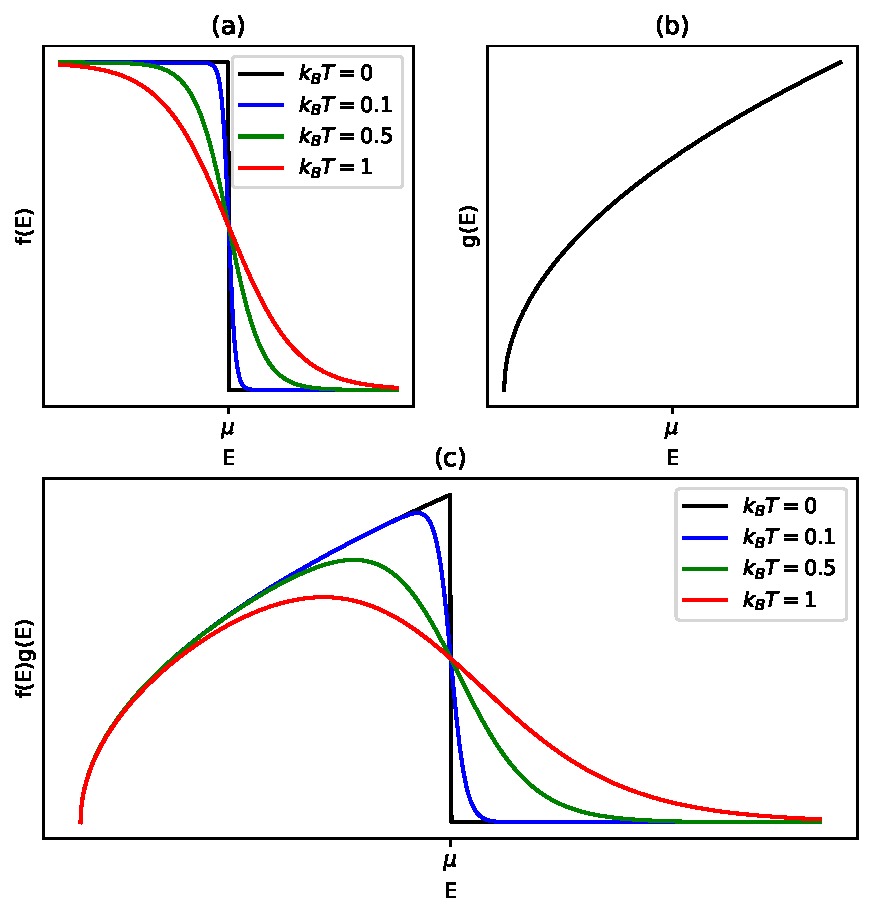
\includegraphics[scale=1]{Imagenes/07-Fermi-function.pdf}
    \caption{(a) representación gráfica de la función $f(E)$; (b) representación gráfica de $g(E)$; (c) representación de $f(E)g(E)$}
    \label{Fig:07-02-01}
\end{figure}

\section{Paramagnetismo de Pauli}
En cada estado $k$ en un metal puede ser doblemente ocupado por cada uno de los espines del electrón. Cuando un campo magnético es aplicado, la energía de cada electrón aumenta o disminuye debido al espín, lo que hace que la densidad de ocupación de uno de los espines sea mas alta que otra, apareciendo una mangnetización no nula y por tanto una suscetibilidad magnética. Este fenómeno es llamado \textbf{paramagnetismo de Pauli}. 

\subsection{Derivación elemental}
En esta sección vamos a despreciar el término orbital ($g=2$ tal que $g \mu_B B = 2 \mu_B B$) y la superficie de Fermi. Lógicamente la magnetización debe venir dada por la diferencia entre número de electrones (por unidad de volumen) con espín hacia arriba $n_\uparrow$ y espines hacia abajo $n_\downarrow$. En ese caso:
\begin{equation}
    M = \mu_B (n_\uparrow - n_\downarrow) 
\end{equation}
Si la diferencia de energía respecto la energía de Fermi $E_F$ es muy pequeña ($\D E = \mu_B B \ll E_F$). Dado que los estados vienen dados por:

\begin{equation}
   \D n = \int g(E) \D E
\end{equation}
En ese caso $n_\uparrow =\frac{1}{2} \parentesis{n_{F} +  g(E_F) \D E}$, de lo que se deduce que

\begin{equation}
    n_\uparrow =  \frac{n_{F}}{2}+ \frac{1}{2} g(E_F) \mu_B B \tquad n_\downarrow = \frac{n_{F}}{2}- \frac{1}{2} g(E_F) \mu_B B
\end{equation}
El factor 1/2 proviene del factor de que ahora no consideramos el caso de dos espines. De no ser así no podría conservarse $n=n_\uparrow + n_\downarrow$. Entonces:

\begin{equation}
    M = g(E_F) \mu_B^2 B
\end{equation}
por lo que si consideramos qeu $\chi_P \approx \mu_0 M /B$ tenemos que

\begin{equation}
    \chi_P = \mu_0 \mu_B^2 g(E_F) = \frac{3 n \mu_0 \mu_B^2}{2 E_F}
\end{equation}
Como podemos ver nuestra expresión del paramagnetismo de Pauli no depende de la temperatura, lo cual no es raro ya que hemos ignorado los fenómenos como el de la superficie de Fermi. El paramagnetismo de Pauli es un efecto muy débil, mucho más pequeño que el observado según la ley de Curie. Esto es porque los aislantes tienen, por lo menos, un electrón en cada átomo que contribuye al fenómeno. En el caso del paramagnetismo de Pauli solo aquellos cerca de la superficie de Pauli juegan un rol en este paramagnetismo. Que el paramagnetismo de Pauli fuera tan pequeño fuera un rompecabezas, hasta que Pauli señalo que era consecuencia de la mecánica de Fermi-Dirac. \\

%\subsection{Relación con el comportamiento localizado}

%En esta sección vamos a estudiar el fenómeno de 

%\section{Bandas espontaneas de espin-zip}

%\section{Teoría de la densidad de espines}

%\section{Diamangetismo de Landau}

%\section{Magnetismo de un gas de electrones}

%\section{Excitaciones en el gas de electrones}

%\section{Ondas de densidad de espin}

%\section{El efecto Kondo}

%\section{El modelo de Hubbard}


%\section{Estrellas de neutrones}
%\newpage
%\chapter{Competencia entre interacciones}




\end{document}